\documentclass[12pt]{article}
\usepackage{graphicx}
\usepackage[margin=2cm]{geometry}
\usepackage[utf8]{inputenc}
\usepackage{tikz}
\usepackage[export]{adjustbox}
\usepackage{indentfirst}
\usepackage{wrapfig}
\usepackage{listings}
\usepackage{color}
\usepackage{enumerate}
\usepackage{amssymb, bm}
\usepackage{csvsimple}
\usepackage{tikz}
\usetikzlibrary{positioning}
\usepackage{lscape}
\newcommand\tab[1][1cm]{\hspace*{#1}}
\definecolor{mygreen}{rgb}{0,0.6,0}
\definecolor{mygray}{rgb}{0.5,0.5,0.5}
\definecolor{mymauve}{rgb}{0.58,0,0.82}
\lstset{ %
    backgroundcolor=\color{gray!10!white},
  basicstyle=\tiny, %footnotesize,        % the size of the fonts that are used for the code
  breakatwhitespace=false,         % sets if automatic breaks should only happen at whitespace
  breaklines=true,                 % sets automatic line breaking
  captionpos=b,                    % sets the caption-position to bottom
  commentstyle=\color{mygreen},    % comment style
  deletekeywords={...},            % if you want to delete keywords from the given language
  escapeinside={\%*}{*)},          % if you want to add LaTeX within your code
  extendedchars=true,              % lets you use non-ASCII characters; for 8-bits encodings only, does not work with UTF-8
  frame=single,	                   % adds a frame around the code
  keepspaces=true,                 % keeps spaces in text, useful for keeping indentation of code (possibly needs columns=flexible)
  keywordstyle=\color{blue},       % keyword style
  language=Python,                 % the language of the code
  morekeywords={*,...},           % if you want to add more keywords to the set
  numbers=left,                    % where to put the line-numbers; possible values are (none, left, right)
  numbersep=10pt,                   % how far the line-numbers are from the code
  numberstyle=\tiny\color{mygray}, % the style that is used for the line-numbers
  rulecolor=\color{black},         % if not set, the frame-color may be changed on line-breaks within not-black text (e.g. comments (green here))
  showspaces=false,                % show spaces everywhere adding particular underscores; it overrides 'showstringspaces'
  showstringspaces=false,          % underline spaces within strings only
  showtabs=false,                  % show tabs within strings adding particular underscores
  stepnumber=1,                    % the step between two line-numbers. If it's 1, each line will be numbered
  stringstyle=\color{mymauve},     % string literal style
  tabsize=1,	                   % sets default tabsize to 2 spaces
  title=\lstname                   % show the filename of files included with \lstinputlisting; also try caption instead of title
}
\graphicspath{ }
\usetikzlibrary{arrows}

\title{\textbf{COMP0086 Summative Assignment}}
%\author{Jian Shu (James) Wu \\ }
\date{Nov 14, 2022}

\begin{document}
\maketitle
\section*{Question 1}


\begin{enumerate}

\item[(a)] Our sample space for images is $\{0, 1\}^D$, where each of our D dimensions can only take binary values (D being the number of pixels in the image).
The exponential family best suited on this sample space is the D-dimensional multivariate Bernoulli distribution because it shares the same sample space.
On the other hand, a D-dimensional multivariate Gaussian has the sample space $\mathbb{R}^D$, which does not match the sample space of our data.
%To match our data sample space, we might have to define an additional mapping between our data and model spaces, adding unnecessary complexity.
It is not immediately clear how the likelihood of an image of binary (discrete) values would be calculated under the continuous distribution of a multivariate Gaussian.
Thus it would be inappropriate to model this dataset of images with a multivariate Gaussian.

\item[(b)] For $\{\textbf{x}^{(n)}\}_{n=1}^N$, a data set of N images, the joint likelihood (assuming images are independently and identically distributed) is the product of N, D-dimensional multivariate Bernoulli distributions:
$$P(\{\textbf{x}^{(n)}\}_{n=1}^N|\textbf{p}) = \prod_{n=1}^N P(\textbf{x}^{(n)} | \textbf{p})$$
Substituting the D-dimensional multivariate Bernoulli:
$$P(\{\textbf{x}^{(n)}\}_{n=1}^N|\textbf{p}) = \prod_{n=1}^{N}\prod_{d=1}^{D} p_d^{x_d^{(n)}} (1-p_d)^{1-x_d^{(n)}}$$
Taking the logarithm, we get the log likelihood:
$$\mathcal{L}(\{\textbf{x}^{(n)}\}_{n=1}^N|\textbf{p}) = \sum_{n=1}^{N}\sum_{d=1}^{D} [x_d^{(n)}\log(p_d) +  (1-x_d^{(n)})\log(1-p_d)]$$
Note that since the logarithm is a monotonically increasing function on $\mathbb{R}_+$, the maximisers and minimisers of the likelihood do not change.
Thus, to solve for the maximum likelihood estimate, $\hat p_d$, we can take the derivative of $\mathcal{L}(\{\textbf{x}^{(n)}\}_{n=1}^N|\textbf{p})$ with respect to $p_d$, the $d^{th}$ element of $\textbf{p}$:
$$\frac{\partial\mathcal{L}(\{\textbf{x}^{(n)}\}_{n=1}^N|\textbf{p})}{\partial p_d} = \sum_{n=1}^{N} (\frac{x_d^{(n)}}{p_d} -  \frac{1-x_d^{(n)}}{1-p_d})$$
$$\frac{\partial\mathcal{L}(\{\textbf{x}^{(n)}\}_{n=1}^N|\textbf{p})}{\partial p_d} = \frac{\sum_{n=1}^{N} x_d^{(n)}}{p_d} -  \frac{\sum_{n=1}^{N} (1-x_d^{(n)})}{1-p_d}$$
and set the derivative to zero to solve for $\hat p_d$:
$$\frac{\sum_{n=1}^{N} x_d^{(n)}}{\hat p_d} -  \frac{\sum_{n=1}^{N} (1-x_d^{(n)})}{1-\hat p_d} = 0$$
$$ \sum_{n=1}^{N} x_d^{(n)} - \hat p_d\sum_{n=1}^{N} x_d^{(n)} - \hat p_d  \cdot N + \hat p_d \sum_{n=1}^{N}x_d^{(n)} = 0$$
$$  \hat p_d = \frac{1}{N}\sum_{n=1}^{N} x_d^{(n)}$$
%Moreover, the second derivative with respect to $p_d$:
%$$\frac{\partial\mathcal{L}(\{\textbf{x}^{(n)}\}_{n=1}^N|\textbf{p})}{\partial p_d^2} = \frac{-\sum_{n=1}^{N} x_d^{(n)}}{p_d^2} +  \frac{-\sum_{n=1}^{N} (1-x_d^{(n)})}{(1-p_d)^2}$$
%For a maximum, we need to show that the second derivative is negative.
%Since $x_d^{(n)} \in \{0, 1\}$, in the worst case, of $N=1$, the single pixel $x_d^{(1)}$ must either be white ($\sum_{n=1}^{N} x_d^{(n)}> 0$) or black ($\sum_{n=1}^{N} 1-x_d^{(n)} > 0$) with the other being zero, so  $\frac{\partial\mathcal{L}(\{\textbf{x}^{(n)}\}_{n=1}^N|\textbf{p})}{\partial p_d^2} < 0$ will be guaranteed and $\hat p_d$ is a maximum as required for the maximum likelihood estimate.

Because we assume that each pixel is independent (we are taking the product of D one dimensional Bernoulli distributions), we can express the maximum likelihood for $\textbf{p}$ in vectorised form as $\hat{\textbf{p}}^{MLE}$:
$$\hat{\textbf{p}}^{MLE} = \frac{1}{N}\sum_{n=1}^{N} \textbf{x}^{(n)}$$

%\item[(c)] Assuming independent Beta priors on the parameters $p_d$:
%
%$$P(p_d) = \frac{1}{B(\alpha, \beta)} p^{\alpha-1}_d (1-p_d)^{\beta-1}$$
%
%and $P(\textbf{p}) = \prod_d P(p_d)$ Find the maximum a posteriori (MAP) estimator for \textbf{p}. [5 marks]

\item[(c)] From Bayes' Theorem:
$$P(\textbf{p}|\{\textbf{x}^{(n)}\}_{n=1}^N) = \frac{ P(\{\textbf{x}^{(n)}\}_{n=1}^N|\textbf{p})P(\textbf{p})}{P(\{\textbf{x}^{(n)}\}_{n=1}^N)}$$
Taking the logarithm:
$$\mathcal{L}(\textbf{p}|\{\textbf{x}^{(n)}\}_{n=1}^N) = \mathcal{L}(\{\textbf{x}^{(n)}\}_{n=1}^N|\textbf{p})+ \mathcal{L}(\textbf{p}) - \mathcal{L}(\{\textbf{x}^{(n)}\}_{n=1}^N)$$
Taking the derivative with respect to $p_d$:
$$\frac{\partial\mathcal{L}(\textbf{p}|\{\textbf{x}^{(n)}\}_{n=1}^N)}{\partial p_d} = \frac{\partial\mathcal{L}(\{\textbf{x}^{(n)}\}_{n=1}^N|\textbf{p})}{\partial p_d} + \frac{\partial\mathcal{L}(\textbf{p})}{\partial p_d}$$
where $\frac{\partial\mathcal{L}(\{\textbf{x}^{(n)}\}_{n=1}^N)}{\partial p_d}$=0 because it doesn't depend on $p_d$.

We know from (b):
$$\frac{\partial\mathcal{L}(\{\textbf{x}^{(n)}\}_{n=1}^N|\textbf{p})}{\partial p_d} = \frac{\sum_{n=1}^{N} x_d^{(n)}}{p_d} -  \frac{\sum_{n=1}^{N} (1-x_d^{(n)})}{1-p_d}$$
For the second term $\frac{\partial\mathcal{L}(\textbf{p})}{\partial p_d}$, we start with $P(\textbf{p})$, assuming each pixel to have an independent prior:
$$P(\textbf{p}) = \prod_{d=1}^D P(p_d)$$
and assuming a Beta prior on each $p_d$:
$$P(\textbf{p}) = \prod_{d=1}^D \frac{1}{B(\alpha, \beta)} p^{\alpha-1}_d (1-p_d)^{\beta-1}$$
Taking the logarithm:
$$\mathcal{L}(\textbf{p}) = \sum_{d=1}^{D} -\log (B(\alpha, \beta)) + (\alpha-1)\log p_d + (\beta-1)\log(1-p_d)$$
Taking the derivative with respect to $p_d$:
$$\frac{\partial\mathcal{L}(\textbf{p})}{\partial p_d} = \frac{(\alpha-1)}{p_d} -  \frac{(\beta-1)}{1-p_d}$$
Since we are only concerned with $p_d$, we are only left with a single element of the summation pertaining to $p_d$.


Combining, we have have an expression for $\frac{\partial\mathcal{L}(\textbf{p}|\{\textbf{x}^{(n)}\}_{n=1}^N)}{\partial p_d}$:
$$\frac{\partial\mathcal{L}(\textbf{p}|\{\textbf{x}^{(n)}\}_{n=1}^N)}{\partial p_d} = \frac{\sum_{n=1}^{N} x_d^{(n)}}{p_d} -  \frac{\sum_{n=1}^{N} (1-x_d^{(n)})}{1-p_d} + \frac{(\alpha-1)}{p_d} -  \frac{(\beta-1)}{1-p_d}$$
$$\frac{\partial\mathcal{L}(\textbf{p}|\{\textbf{x}^{(n)}\}_{n=1}^N)}{\partial p_d} = \frac{(\alpha-1) + \sum_{n=1}^{N} x_d^{(n)}}{p_d} -  \frac{(\beta-1) + \sum_{n=1}^{N} (1-x_d^{(n)})}{1-p_d}$$
To find the maximum a posteriori (MAP) estimate $\hat{p_d}$ set $\frac{\partial\mathcal{L}(\textbf{p}|\{\textbf{x}^{(n)}\}_{n=1}^N)}{\partial p_d} = 0$ and solve:
$$0 = \frac{(\alpha-1) + \sum_{n=1}^{N} x_d^{(n)}}{\hat{p_d}} -  \frac{(\beta-1) + \sum_{n=1}^{N} (1-x_d^{(n)})}{1-\hat{p_d}}$$
$$0 = (1-\hat{p_d})(\alpha-1) + (1-\hat{p_d})\bigg(\sum_{n=1}^{N} x_d^{(n)}\bigg) -  \hat{p_d}(\beta-1) - \hat{p_d}\bigg(\sum_{n=1}^{N} (1-x_d^{(n)})\bigg)$$
$$0 = (\alpha-\alpha \hat{p_d} + \hat{p_d} - 1) +\bigg(\sum_{n=1}^{N} x_d^{(n)} - \hat{p_d} \sum_{n=1}^{N} x_d^{(n)}\bigg) -  (\hat{p_d}\beta-\hat {p_d}) - \bigg(\hat{p_d}\cdot N - \hat{p_d}\sum_{n=1}^{N}x_d^{(n)}\bigg)$$
Cancelling the $\hat p_d\sum_{n=1}^{N} x_d^{(n)}$ terms:
$$0 = \alpha-\alpha \hat{p_d} + \hat{p_d} - 1 +\sum_{n=1}^{N} x_d^{(n)} -  \hat{p_d}\beta+\hat{p_d} - \hat{p_d}\cdot N$$
$$0 = \hat{p_d}(2-\alpha-\beta-N) + \alpha - 1 +\sum_{n=1}^{N} x_d^{(n)}$$
$$\hat{p_d} =  \frac{\alpha - 1 +\sum_{n=1}^{N} x_d^{(n)}}{(N+\alpha+\beta-2)}$$
%To show that this is a maximum, the second derivative is:
%$$\frac{\partial^2\mathcal{L}(\textbf{p}|\{\textbf{x}^{(n)}\}_{n=1}^N)}{(\partial p_d)^2} = \frac{(1-\alpha) - \sum_{n=1}^{N} x_d^{(n)}}{(p_d)^2} +  \frac{(1-\beta) - \sum_{n=1}^{N} (1-x_d^{(n)})}{(1-p_d)^2}$$.
%For a maximum, we need $\frac{\partial^2\mathcal{L}(\textbf{p}|\{\textbf{x}^{(n)}\}_{n=1}^N)}{(\partial p_d)^2} < 0$ meaning that we need at least one of the strict inequalities $\alpha < 1- \sum_{n=1}^{N} x_d^{(n)}$ or $\beta < 1-\sum_{n=1}^{N} (1-x_d^{(n)})$ to be satisified, where the other can be $\leq$. The Beta distribution requires $\alpha > 0$ and $\beta > 0$ so this requirement will always be satisfied (in the worst case of a single image, either $x_d^{(1)}=1$ or $1-x_d^{(1)}=1$).

Due to independence of our likelihood and priors for each dimension, we can express the maximum a priori for \textbf{p} in vectorised form as $\hat{\textbf{p}}^{MAP}$:
$$\hat{\textbf{p}}^{MAP} =   \frac{\alpha - 1 +\sum_{n=1}^{N} \textbf{x}^n}{(N+\alpha+\beta-2)}$$


\newpage
\item[(d\&e)] The Python code for MLE and MAP:
\lstinputlisting[language=Python, caption: MLE and MAP Implementation,]{src/solutions/q1.py}
\newpage
%  \begin{figure}[h]
%  \centering
%  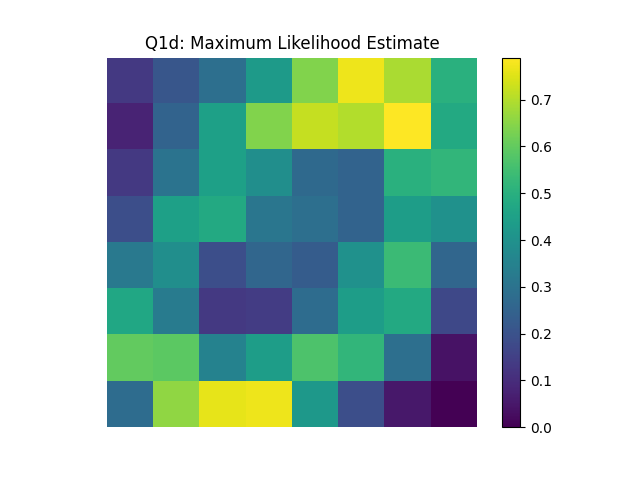
\includegraphics[scale=0.5]{outputs/q1/q1d}
%  \caption{ML parameters}
%  \label{fig:1d}
%  \end{figure}
%  \begin{figure}[h]
%  \centering
%  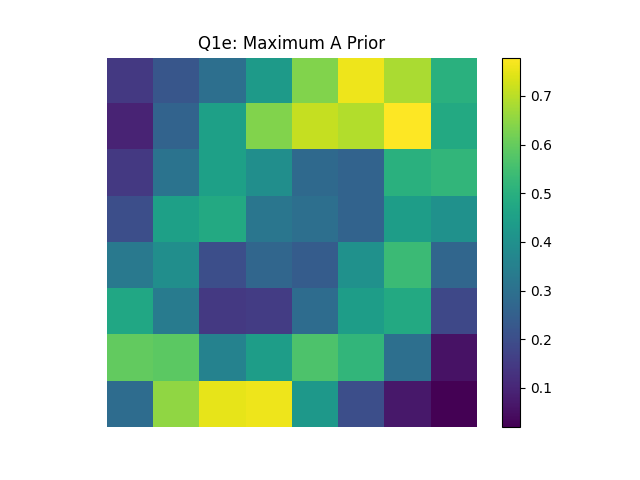
\includegraphics[scale=0.5]{outputs/q1/q1e}
%  \caption{MAP parameters}
%  \label{fig:1e}
%  \end{figure}

Displaying the learned parameters:
\begin{figure}[h]
\centering
\begin{minipage}{0.5\textwidth}
  \centering
  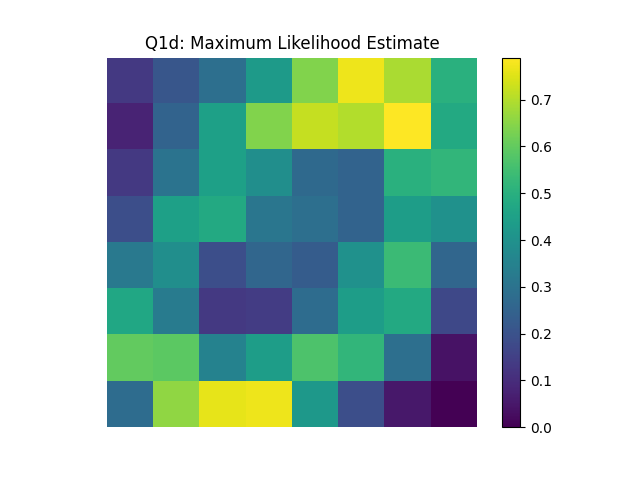
\includegraphics[scale=0.4]{outputs/q1/q1d}
  \caption{ML parameters}
  \label{fig:1d}
\end{minipage}%
\begin{minipage}{0.5\textwidth}
  \centering
  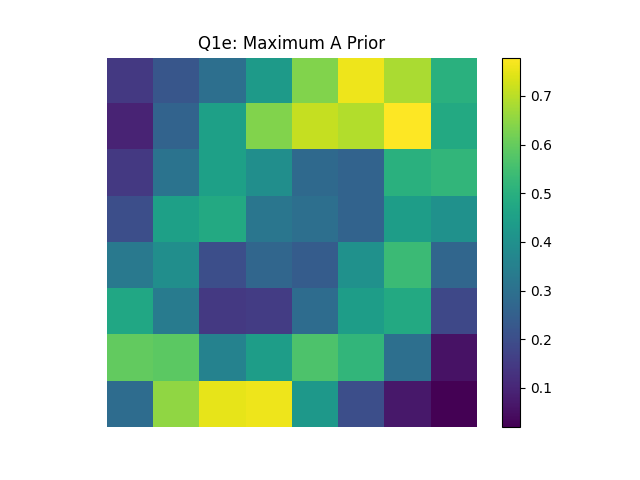
\includegraphics[scale=0.4]{outputs/q1/q1e}
  \caption{MAP parameters}
  \label{fig:1e}
\end{minipage}
\end{figure}

Comparing the equations:
    $$\hat{\textbf{p}}^{MLE} = \frac{1}{N}\sum_{n=1}^{N} \textbf{x}^{(n)}$$
    and
    $$\hat{\textbf{p}}^{MAP}  =  \frac{\alpha - 1 +\sum_{n=1}^{N} \textbf{x}^n}{(N+\alpha+\beta-2)}$$
As the number of data points increases, $\hat{\textbf{p}}^{MAP}$ approaches $\frac{1}{N}\sum_{n=1}^{N} \textbf{x}^{(n)}$, the $\hat{\textbf{p}}^{MLE}$.
This makes sense because as our data set gets bigger, the effect of the prior diminishes.
However, if a specific pixel in all of the images of our data set are white or all black, the MLE for that pixel would either be 1 or 0.
This may not be representative of our intuitions about images, as there should be some non-zero probability of a pixel being black or white.
By introducing an appropriate prior we can ensure that the probability of that pixel will never be exactly zero or one.
In our case, with a Beta(3,3) prior on each pixel, our parameter values are biased to be closer to 0.5 and to never be at the extremities 0 and 1.
We can see this in Figure $\ref{fig:1e}$ where the range of our parameters is smaller than the range of Figure $\ref{fig:1d}$ and doesn't include zero.
Figure $\ref{fig:1e-comparison}$ visualises $\hat{\textbf{p}}^{MAP}-\hat{\textbf{p}}^{MLE}$ and we can see that for likelihoods greater than 0.5 in the MLE, the MAP has a lower value and for likelihoods less than 0.5, the MAP has a higher value, confirming our intuitions.

  \begin{figure}[h]
  \centering
  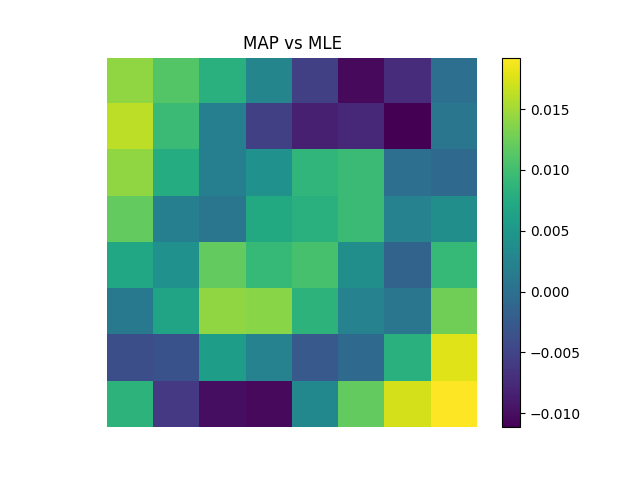
\includegraphics[scale=0.4]{outputs/q1/q1e-mle-vs-map}
  \caption{$\hat{\textbf{p}}^{MAP}-\hat{\textbf{p}}^{MLE}$}
  \label{fig:1e-comparison}
  \end{figure}

Priors can also help ensure numerical stability during calculations.
The logarithm of zero is negative infinity, so having if the MLE is zero it can be problematic for log-likelihood calculations whereas MAP can ensure non-zero probabilities.
Interestingly, when $\alpha=\beta=1$, $\hat{\textbf{p}}^{MLE} = \hat{\textbf{p}}^{MAP}$.
This is when the prior is a uniform distribution and so there is uniform bias on the location of $\textbf{p}$ and we recover the MLE.

On the other hand, a mis-specified prior can be problematic, as the estimated parameters might be skewed by the prior and not properly represent the underlying data generating process, this can result in parameter estimates that are `worse' than using the MLE if our data set is limited in size.
%In this example, we're using images of different digits as part of our data set. If a particular digit occurs more frequently in the data set, we will see that digit when visualising the MLE or MAP (the digit zero in this case), they simply provides the "average" image pixels. With a set of images with more equal representation of each digit, the parameter visualisation could be an image overlaying the different digits, which is not representative of the "most likely" image in the data. In this case where our data is likely clustered, using a multimodal likelihood is probably a better idea than the unimodal likelihood we've used.



%With MAP, if we have priors skewed towards the parameters for under represented digits in our data, it is more likely to "even out" the estimated parameters. In our case, we used the same Beta prior on all pixels, essentially placing a "uniform shading" on the entire image, so we could not




\end{enumerate}

\newpage
\section*{Question 2}

\item[] When all D components are generated from a Bernoulli distribution with $p_d = 0.5$, we have the likelihood function for model $M_1$:
$$P(\{\textbf{x}^{(n)}\}_{n=1}^{N}|\textbf{p}^{(1)}}=[0.5, 0.5,...,0.5]^T, M_1) = \prod_{n=1}^{N}\prod_{d=1}^{D} (0.5)^{x_d^{(n)}} (0.5)^{1-x_d^{(n)}}$$
Knowing that either $x_d^{(n)}$ or $1-x_d^{(n)}$ will be 1 and the other zero, we can simplify $(0.5)^{x_d^{(n)}} (1-0.5)^{1-{x_d}^{(n)}}$ to $0.5$:
$$P(\{\textbf{x}^{(n)}\}_{n=1}^{N}|\textbf{p}^{(1)}}=[0.5, 0.5,...,0.5]^T, M_1) = \prod_{n=1}^{N} \prod_{d=1}^D (0.5)$$
$$P(\{\textbf{x}^{(n)}\}_{n=1}^{N}|\textbf{p}^{(1)}}=[0.5, 0.5,...,0.5]^T, M_1) = 0.5^{N\cdot D}$$
When all D components are generated from Bernoulli distributions with unknown, but identical, $p_d$, we have the likelihood function for model $M_2$:
$$P(\{\textbf{x}^{(n)}\}_{n=1}^{N}|\textbf{p}^{(2)}}=[p_d, p_d, ..., p_d]^T, M_2) = \prod_{n=1}^{N}\prod_{d'=1}^{D} p_d^{x_{d'}^{(n)}} (1-p_d)^{1-x_{d'}^{(n)}}$$
When each component is Bernoulli distributed with separate, unknown $p_d$, we have the likelihood function for model $M_3$:
$$P(\{\textbf{x}^{(n)}\}_{n=1}^{N}|\textbf{p}^{(3)}}=[p_1, p_2, ..., p_D]^T, M_3) = \prod_{n=1}^{N}\prod_{d=1}^{D} p_d^{x_d^{(n)}} (1-p_d)^{1-x_d^{(n)}}$$
For each model $M_i$, we can marginalise out $\textbf{p}^{(i)}}$ to get $P( \{\textbf{x}^{(n)}\}_{n=1}^{N}|M_i)$:
$$P( \{\textbf{x}^{(n)}\}_{n=1}^{N}|M_i) = \int_0^1...\int_0^1 P( \{\textbf{x}^{(n)}\}_{n=1}^{N}|\textbf{p}^{(i)}, M_i)P(\textbf{p}^{(i)}|M_i) dp_1...dp_D$$
Given that the prior of any unknown probabilities is uniform, i.e. $P(\textbf{p}^{(i)} | M_i) = 1$. We can simplify:
$$P( \{\textbf{x}^{(n)}\}_{n=1}^{N}|M_i) = \int_0^1...\int_0^1 P(\{\textbf{x}^{(n)}\}_{n=1}^{N}|\textbf{p}^{(i)}, M_i) dp_1...dp_D$$
For $M_1$:
$$P( \{\textbf{x}^{(n)}\}_{n=1}^{N}|M_1) = \int_0^1...\int_0^1 0.5^{N\cdot D} d\theta_1...d\theta_D$$
We can remove the integrals:
$$P( \{\textbf{x}^{(n)}\}_{n=1}^{N}|M_1) = (0.5)^{N\cdot D}$$
For $M_2$, we have that all pixels share some probability $p_d$ so we only need to integrate over a single variable $p_d$:
$$P( \{\textbf{x}^{(n)}\}_{n=1}^{N}|M_2) = \int_0^1 \prod_{n=1}^{N} \prod_{d'=1}^D p_d^{x_{d'}^{(n)}} (1-p_d)^{1-{x_{d'}}^{(n)}} dp_d$$
Changing the products to sums:
$$P( \{\textbf{x}^{(n)}\}_{n=1}^{N}|M_2) = \int_0^1  p_d^{\sum_{n=1}^{N} \sum_{d'=1}^D x_{d'}^{(n)}} (1-p_d)^{\sum_{j=1}^{N} \sum_{d'=1}^D 1-{x_{d'}^{(n)}}} d p_d$$
Rewriting:
$$P( \{\textbf{x}^{(n)}\}_{n=1}^{N}|M_2) = \int_0^1  (p_d)^{K} (1- p_{d'=1})^{N\cdot D-K} d p_d$$
where $K =\sum_{n=1}^{N} \sum_{d'=1}^D x_{d'}^{(n)}$.

\item[]This integral is the beta function:
$$P( \{\textbf{x}^{(n)}\}_{n=1}^{N}|M_2) = \frac{K! (N\cdot D-K)!}{(N\cdot D+1)!}$$
For $M_3$, we need an integral for each $p_d$:
$$P( \{\textbf{x}^{(n)}\}_{n=1}^{N}|M_3) = \int_0^1 ... \int_0^1 \prod_{n=1}^{N} \prod_{d=1}^D  p_d^{x_d^{(n)}} (1- p_d)^{1-{x_d}^{(n)}} d p_1 ... d p_D$$
We can separate the integrals to only contain the relevant $p_d$:
$$P( \{\textbf{x}^{(n)}\}_{n=1}^{N}|M_3) = \prod_{d=1}^D \Bigg( \int_0^1 \prod_{n=1}^{N}   p_d^{x_d^{(n)}} (1- p_d)^{1-{x_d}^{(n)}} d p_d \Bigg)$$
Changing the products to sums:
$$P( \{\textbf{x}^{(n)}\}_{n=1}^{N}|M_3) = \prod_{d=1}^D \Bigg( \int_0^1   p_d^{\sum_{n=1}^{N} x_d^{(n)}} (1- p_d)^{\sum_{n=1}^{N} 1-{x_d}^{(n)}} d p_d \Bigg)$$
In this case, we have the product of integrals where each evaluates to a beta function:
$$P( \{\textbf{x}^{(n)}\}_{n=1}^{N}|M_3) = \prod_{d=1}^D \frac{K_d! (N-K_d)!}{(N+1)!}$$
where $K_d = \sum_{n=1}^{N} x_d^{(n}$.

\item[]The posterior probability of a model $M_i$ can be expressed:
$$P(M_i |  \{\textbf{x}^{(n)}\}_{n=1}^{N}) = \frac{P( \{\textbf{x}^{(n)}\}_{n=1}^{N}|M_i)P(M_i)}{P( \{\textbf{x}^{(n)}\}_{n=1}^{N})}$$
We only have three models, so in this case the normalisation $P(\{\textbf{x}^{(n)}\}_{n=1}^{N})$ can be expressed as a sum:
$$P(M_i| \{\textbf{x}^{(n)}\}_{n=1}^{N}) = \frac{P( \{\textbf{x}^{(n)}\}_{n=1}^{N}|M_i)P(M_i)}{\sum_{i\in \{1,2,3\}} P( \{\textbf{x}^{(n)}\}_{n=1}^{N}|M_i)P(M_i)}$$
Given that $P(M_i) = \frac{1}{3}$ for all $i \in \{1,2,3\}$:
$$P(M_i| \{\textbf{x}^{(n)}\}_{n=1}^{N}) = \frac{P( \{\textbf{x}^{(n)}\}_{n=1}^{N}|M_i)}{\sum_{i\in \{1,2,3\}} P( \{\textbf{x}^{(n)}\}_{n=1}^{N}|M_i)}$$
\newpage
Calculating the posterior probabilities of each of the three models having generated the data in binarydigits.txt using Python, we can show the values in the Table $\ref{table2}$.

\begin{table}[h]
\begin{center}

\begin{tabular}{l|c}%

 \bfseries $i$ & \bfseries$ P(M_i|\{\textbf{x}^{(n)}\}_{n=1}^{N})$% specify table head
\csvreader[head to column names]{outputs/q2/q2c.csv}{}% use head of csv as column names
{\\\hline\csvcoli&\csvcolii}% specify your coloumns here
\end{tabular}
\end{center}
\caption{Posterior Probabilities}
\label{table2}
\end{table}

We can see that for models specified to have the same parameter value for all pixels, like $M_1$, is very unlikely with the given data set. This makes sense because it is specifying models where the image is essentially blank (a uniform shade), which is not reflective of our digit images. Moreover, $M_1$ specifies a specific value of 0.5 for all the parameters whereas $M_2$ specifies any value for all the parameters as long as it's the same. So the model $M_1$ is just one possible model specified in $M_2$ and we can see this reflected in our probabilities when $P(M_2|\{\textbf{x}^{(n)}\}_{n=1}^{N}) > P(M_1|\{\textbf{x}^{(n)}\}_{n=1}^{N})$.

\newpage
The Python code for calculating the posterior probabilities of the three models:
\lstinputlisting[language=Python]{src/solutions/q2.py}
\newpage
\section*{Question 3}

\begin{enumerate}

%\item[(a)] Write down the likelihood for a model consisting of a mixture of K multivariate Bernoulli
%distributions. Use the parameters $\pi_1, . . . , \pi_K$ to denote the mixing proportions $(0 \leq \pi_k \leq 1; \sum_k \pi_k = 1)$ and arrange the K Bernoulli parameter vectors into a matrix P with elements
%$p_{kd}$ denoting the probability that pixel d takes value 1 under mixture component k. Assume the images are iid under the model, and that the pixels are independent of each other within each component distribution. [5 marks]
%
%
%Just as we can for a mixture of Gaussians, we can formulate this mixture as a latent variable
%model, introducing a discrete hidden variable $s(n) \in \{1, . . . , K \}$ where $P (s(n) = k|\pi) = \pi_k$.

\item[(a)] The likelihood for a model consisting of a mixture of K multivariate Bernoulli distributions can be expressed as the product across $N$ data points:
$$P(\{\textbf{x}^{(n)}\}_{n=1}^{N}|\theta) = \prod_{i=1}^{N}P(\textbf{x}^{(n)}|\theta)$$
where $\{\textbf{x}^{(n)}\}_{n=1}^{N}$ is our data set with $\textbf{x}^{(n)} \in \mathbb{R}^{D \times 1}$ and $\theta = \{\pi, \mathbf{P}\}$ are our parameters, $\pi = [\pi_1, . . . , \pi_K] \in \mathbb{R}^{K \times 1}$ our K mixing proportions $(0 \leq \pi_k \leq 1; \sum_k \pi_k = 1)$ and $\mathbf{P} \in \mathbb{R}^{D \times K}$ the K Bernoulli parameter vectors with elements $p_{kd}$ denoting the probability that pixel d takes value 1 given mixture component k. We also assume the images are iid and that the pixels are independent of each other within each component distribution.

For each $P(\textbf{x}^{(n)}|\theta)$:
$$P(\textbf{x}^{(n)}|\theta) = \sum_{k=1}^{K} \pi_k \prod_{d=1}^D (p_{kd})^{x^{(n)}_{d}} (1-p_{kd})^{1-x^{(n)}_{d}}$$
The log-likelihood $\mathcal{L}(\textbf{x}^{(n)}|\theta)$ can be expressed in vector form:
$$\mathcal{L}(\textbf{x}^{(n)}|\theta) = \log \sum_{k=1}^{K}  \pi_k \exp\bigg(\textbf{x}^{(n)}\log(\mathbf{P}_{k}) + (1-\textbf{x}^{(n)})\log(1-\mathbf{P}_{k})\bigg) $$
which can be further vectorised using Python scipy's $logsumexp$ operation.

Moreover, the log-likelihood $\mathcal{L}(\{\textbf{x}^{(n)}\}_{n=1}^{N}|\theta)$ can be expressed:
$$\mathcal{L}(\{\textbf{x}^{(n)}\}_{n=1}^{N}|\theta) = \sum_{i=1}^{N} \Bigg( \log \sum_{k=1}^{K}  \pi_k \exp\bigg(\textbf{x}^{(n)}\log(\mathbf{P}_{k}) + (1-\textbf{x}^{(n)})\log(1-\mathbf{P}_{k})\bigg) \Bigg)$$

\item[(b)] We know that:
$$P(A|B) \propto P(B|A)P(A)$$
Thus,
$$P(s^{(n)} = k|\textbf{x}^{(n)}, \pi, \mathbf{P}) \propto  P(\textbf{x}^{(n)} | s^{(n)} = k, \pi, \mathbf{P}) P(s^{(n)} = k|\pi, \mathbf{P})$$
where $s^{(n)} \in \{1,...,K\}$ a discrete hidden variable with $P(s^{(n)} = k|\textbf{x}^{(n)}, \pi) = \pi_k$. Note that $P(s^{(n)} = k|\pi, \mathbf{P}) = P(s^{(n)} = k| \pi)$ as $s^{(n)$ isn't dependent on $\mathbf{P}$.

Let $\tilde{r}_{nk}$ be the unnormalised responsibility $ P(\textbf{x}^{(n)} | s^{(n)} = k, \pi, \mathbf{P}) P(s^{(n)} = k|\pi, \mathbf{P})$. Using the mixture for component $k$, $\pi_k$ and the likelihood function of component $k$:
$$\tilde{r}_{nk} = \pi_k \prod_{d=1}^D (p_{kd})^{x^{(n)}_{d}} (1-p_{kd})^{1-x^{(n)}_{d}}$$
Normalising across the components:
$$r_{nk} = \frac{\tilde{r}_{nk}}{\sum_{j=1}^K\tilde{r}_{nj}}$$
we have calculated $P(s^{(n)} = k|\textbf{x}^{(n)}, \pi, \mathbf{P})$ for the E step of an EM algorithm.

Moreover,
$$ \log \tilde{r}_{nk} = \log \pi_k + \sum_{d=1}^D \bigg( x^{(n)}_{d}\log(p_{kd}) + (1-x^{(n)}_{d}) \log(1-\exp(\log(p_{kd}))) \bigg)$$
and
$$\log r_{nk} = \log\tilde{r}_{nk} - \log\sum_{j=1}^K\exp(\log\tilde{r}_{nj})$$
which can be vectorised as $\log \textbf{r}$ calculated with $\log\pi$ and $\log \textbf{P}$ using Python scipy's $logsumexp$ operation.

\item[(c)] We know that the expectation log joint can be expressed:
$$\Bigg\langle \sum_n \log P(\textbf{x}^{(n)}, s^{(n)}| \pi, \mathbf{P})\Bigg\rangle_{q(\{s^{(n)}\})} = \sum_{n=1}^N q(s^{(n)}) \log P(\textbf{x}^{(n)}, s^{(n)}| \pi, \mathbf{P})$$
Let this quantity be $E$. For each term of $E$:
$$q(s^{(n)}) = \textbf{r}_{n}^T$$
and
$$\log P(\textbf{x}^{(n)}, s^{(n)}| \pi, \mathbf{P}) = \log[P(\textbf{x}^{(n)}| s^{(n)}, \pi, \mathbf{P})P(s^{(n)}| \pi, \mathbf{P})]$$
which is the vectorised version of $\log\tilde{r}_{nk}$ from part (b) so:
$$\log P(\textbf{x}^{(n)}, s^{(n)}| \pi, \mathbf{P}) =\log(\pi)+\log(\mathbf{P})^T \textbf{x}^{(n)} + \log(1-\mathbf{P})^T(1-\textbf{x}^{(n)})$$
Combining:
$$ E = \sum_n \textbf{r}_{n}^T[\log(\pi)+\log(\mathbf{P})^T \textbf{x}^{(n)} + \log(1-\mathbf{P})^T(1-\textbf{x}^{(n)})]$$
To maximise with respect to $\pi$ and $\mathbf{P}$ for the M step, we want to take the derivative, set to zero, and solve for $\hat\pi$ and $\hat \textbf{P}$.

For the $k^{th}$ element of $\pi$:
$$\frac{\partial E}{\partial \pi_k} = \sum_n r_{nk} \frac{1}{\pi_k}$$
%The second derivative:
%$$\frac{\partial E}{(\partial \pi_k)^2} = \sum_n r_{nk} \frac{-1}{(\pi_k)^2}$$
%is always negative because $r_{nk}\geq 0$, $\sum_{n}r_{nk}=1$, \pi_{k}\geq 0$, and $\sum_{n}\pi_{k}=1$, ensuring a maximum in the next step.

We can calculate the maximiser with:
$$\frac{\partial E}{\partial \pi_k} + \lambda = 0$$
where $\lambda$ is a Lagrange multiplier ensuring that the mixing proportions sum to unity.

Thus,
$$\hat \pi_k = \frac{\sum_{n}r_{nk}}{N}$$
For the $dk^{th}$ element of $\mathbf{P}$:
$$\frac{\partial E}{\partial \mathbf{P}_{dk}} = \sum_n r_{nk}\frac{\partial}{\partial \mathbf{P}_{dk}}[x^{(n)}_{d}\log \mathbf{P}_{dk}+(1-x^{(n)}_{d}) \log(1-\mathbf{P}_{dk})]$$
Simplifying:
$$\frac{\partial E}{\partial \mathbf{P}_{dk}} = \sum_n r_{nk}(\frac{x^{(n)}_{d}}{ \mathbf{P}_{dk}}-\frac{1-x^{(n)}_{d}}{1-\mathbf{P}_{dk}})$$
%Similar to Question 1, we can see that taking second derivative, the term in the brackets will always be less than zero and with $r_{nk}\geq 0$ and $\sum_{n}r_{nk}=1$, the second derivative will always be negative. This ensures that we have a maximum in the next step.

Setting the derivative to zero:
$$\frac{\sum_n  x^{(n)}_{d}r_{nk}}{\hat{\mathbf{P}}_{dk}}-\frac{\sum_n r_{nk}-\sum_n  x^{(n)}_{d}r_{nk}}{1-\hat{\mathbf{P}}_{dk}} = 0$$
Solving for $\hat{\mathbf{P}}_{dk}$:
$$\hat{\mathbf{P}}_{dk}\sum_n r_{nk}-\hat{\mathbf{P}}_{dk}\sum_n x^{(n)}_{d}r_{nk} = \sum_n  x^{(n)}_{d}r_{nk}-\hat{\mathbf{P}}_{dk}\sum_n  x^{(n)}_{d}r_{nk}$$
Thus,
$$\hat{\mathbf{P}}_{dk} = \frac{\sum_n x^{(n)}_{d}r_{nk}}{\sum_n r_{nk}}$$
We have the maximizing parameters for the expected log-joint
$$\arg \max_{\pi, \mathbf{P}} \Bigg\langle \sum_n \log P(\textbf{x}^{(n)}, s^{(n)}| \pi, \mathbf{P})\Bigg\rangle_{q(\{s^{(n)}\})}$$
thus obtaining an iterative update for the parameters $\pi$ and $\mathbf{P}$ in the M-step of EM.

\item[]For numerical stability, we can compute the maximisation step for the MAP of $\mathbf{P}$, by solving for $\hat{\mathbf{P}}_{dk}^{MAP}$ with:
$$\frac{\partial E'}{\partial \mathbf{P}_{dk}} = 0$$
where
$$E' = \sum_{n=1}^N q(s^{(n)}) \log P(\mathbf{P} | \pi, \textbf{x}^{(n)}, s^{(n)})$$
and from Bayes':
$$\log P(\mathbf{P} | \pi, \textbf{x}^{(n)}, s^{(n)}) = \log P( \textbf{x}^{(n)}, s^{(n)} | \pi, \mathbf{P} ) + \log P(\mathbf{P}) - \log P(\textbf{x}^{(n)}, s^{(n)} | \pi)$$
Assuming an independent Beta prior on each pixel of each component:
$$\log P(\mathbf{P}) = \sum_{k=1}^K \sum_{d=1}^D -\log (B(\alpha, \beta)) + (\alpha-1)\log \mathbf{P}_{dk} + (\beta-1)\log(1-\mathbf{P}_{dk})$$
and
$$\frac{\partial \log P(\mathbf{P})}{\partial \mathbf{P}_{dk}} = \frac{(\alpha-1)}{\mathbf{P}_{dk}} -  \frac{(\beta-1)}{1-\mathbf{P}_{dk}}$$
Thus, the derivative can be expressed as:
$$\frac{\partial E'}{\partial \mathbf{P}_{dk}} =  \sum_n \Bigg(r_{nk} \bigg(\frac{\partial \log P( \textbf{x}^{(n)}, s^{(n)} | \pi, \mathbf{P} )}{\partial \mathbf{P}_{dk}} + \frac{\partial \log P(\mathbf{P})}{\partial \mathbf{P}_{dk}} \bigg) \Bigg)$$
Substituting the appropriate expressions:
$$\frac{\partial E'}{\partial \mathbf{P}_{dk}} =  \sum_n \Bigg(r_{nk} \bigg(\frac{x^{(n)}_{d}}{ \mathbf{P}_{dk}}-\frac{1-x^{(n)}_{d}}{1-\mathbf{P}_{dk}} + \frac{(\alpha-1)}{\mathbf{P}_{dk}} -  \frac{(\beta-1)}{1-\mathbf{P}_{dk}} \bigg) \Bigg)$$
Simplifying:
$$\frac{\partial E'}{\partial \mathbf{P}_{dk}} =  \frac{\sum_n r_{nk}(\alpha-1 + x^{(n)}_{d})}{ \mathbf{P}_{dk}}-\frac{\sum_n r_{nk}(\beta-x^{(n)}_{d})}{1-\mathbf{P}_{dk}}$$
%For a maximum, we see that we need $\alpha > x^{(n)}_{d}-1$  or $\beta < x^{(n)}_{d}$, both of which are satisfied knowing that $\alpha > 0$ and $\beta > 0$.
Setting $\frac{\partial E'}{\partial \mathbf{P}_{dk}}=0$ we can calculate $\hat{\mathbf{P}}_{dk}^{MAP}$:
$$\sum_n r_{nk}(\alpha-1 + x^{(n)}_{d})} - \hat{\mathbf{P}}_{dk}\sum_n r_{nk}(\alpha-1 + x^{(n)}_{d})} = \hat{\mathbf{P}}_{dk}\sum_n r_{nk}(\beta-x^{(n)}_{d})$$
$$ \hat{\mathbf{P}}_{dk}^{MAP} = \frac{\sum_n r_{nk}(x^{(n)}_{d}+\alpha-1)}{(\alpha+\beta-1)( \sum_n r_{nk})}$$
As a sense check, we can see when setting $\alpha=1$ and $\beta=1$ we recover $ \hat{\mathbf{P}}_{dk}^{MLE}$ as we would expect. For the following parts, a very weak Beta(1+1e-5, 1+1e-5) prior was used.
\newpage
\item[(d)] Plotting the unnormalised posterior likelihood as a function of the iteration number for different k values:

\begin{figure}[h]
\centering
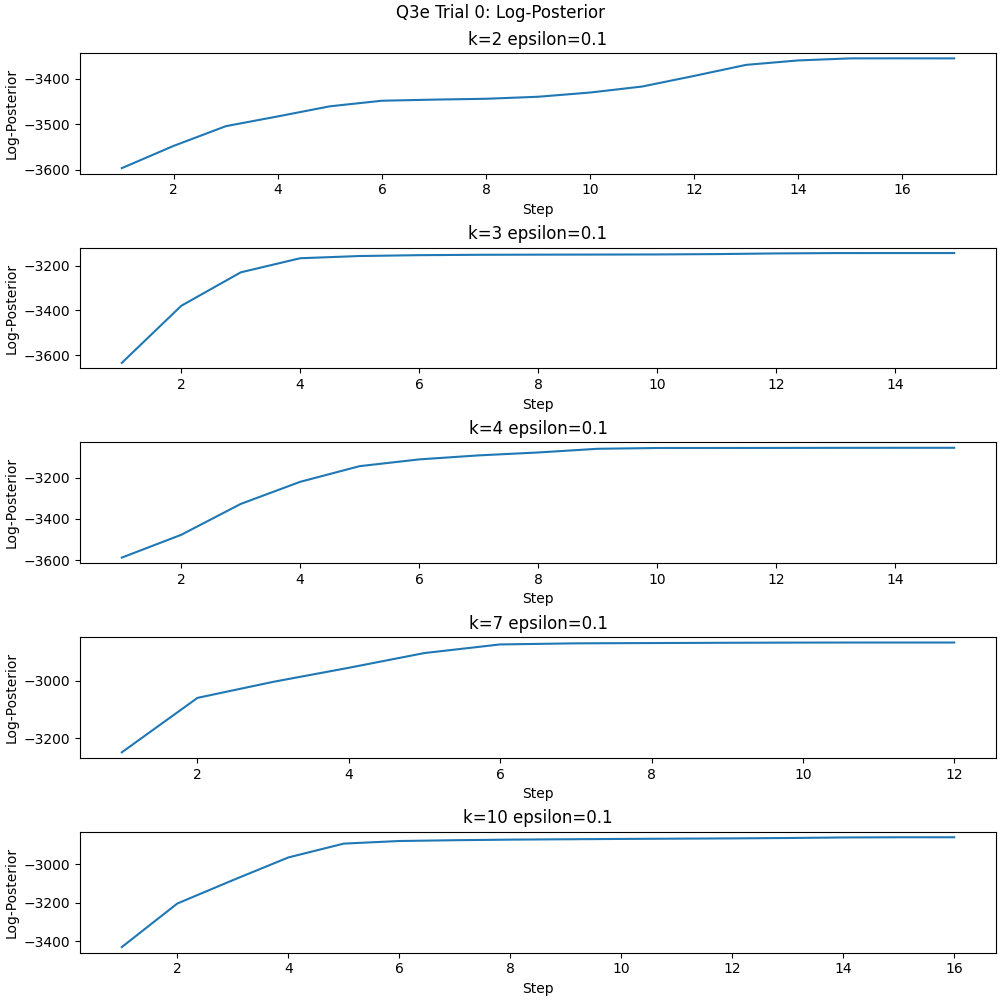
\includegraphics[scale=0.35]{outputs/q3/q3e-0-log-pos}
\caption{Unnormalised Log Posterior vs Iteration Number}
\label{fig:3d-log-like}
\end{figure}

where $epsilon$ is the stopping condition for when the unnormalised log posterior converges sufficiently. Note that the normalisation constant for the log posterior $\log P(\textbf{x}^{(n)}, s^{(n)} | \pi)$ is intractable and so only the unnormalised portion $\log P( \textbf{x}^{(n)}, s^{(n)} | \pi, \mathbf{P} ) + \log P(\mathbf{P})$ was computed and reported.

\newpage

Displaying the parameters found for $K \in \{2, 3, 4, 7, 10\}$:
\begin{figure}[h]
  \centering
  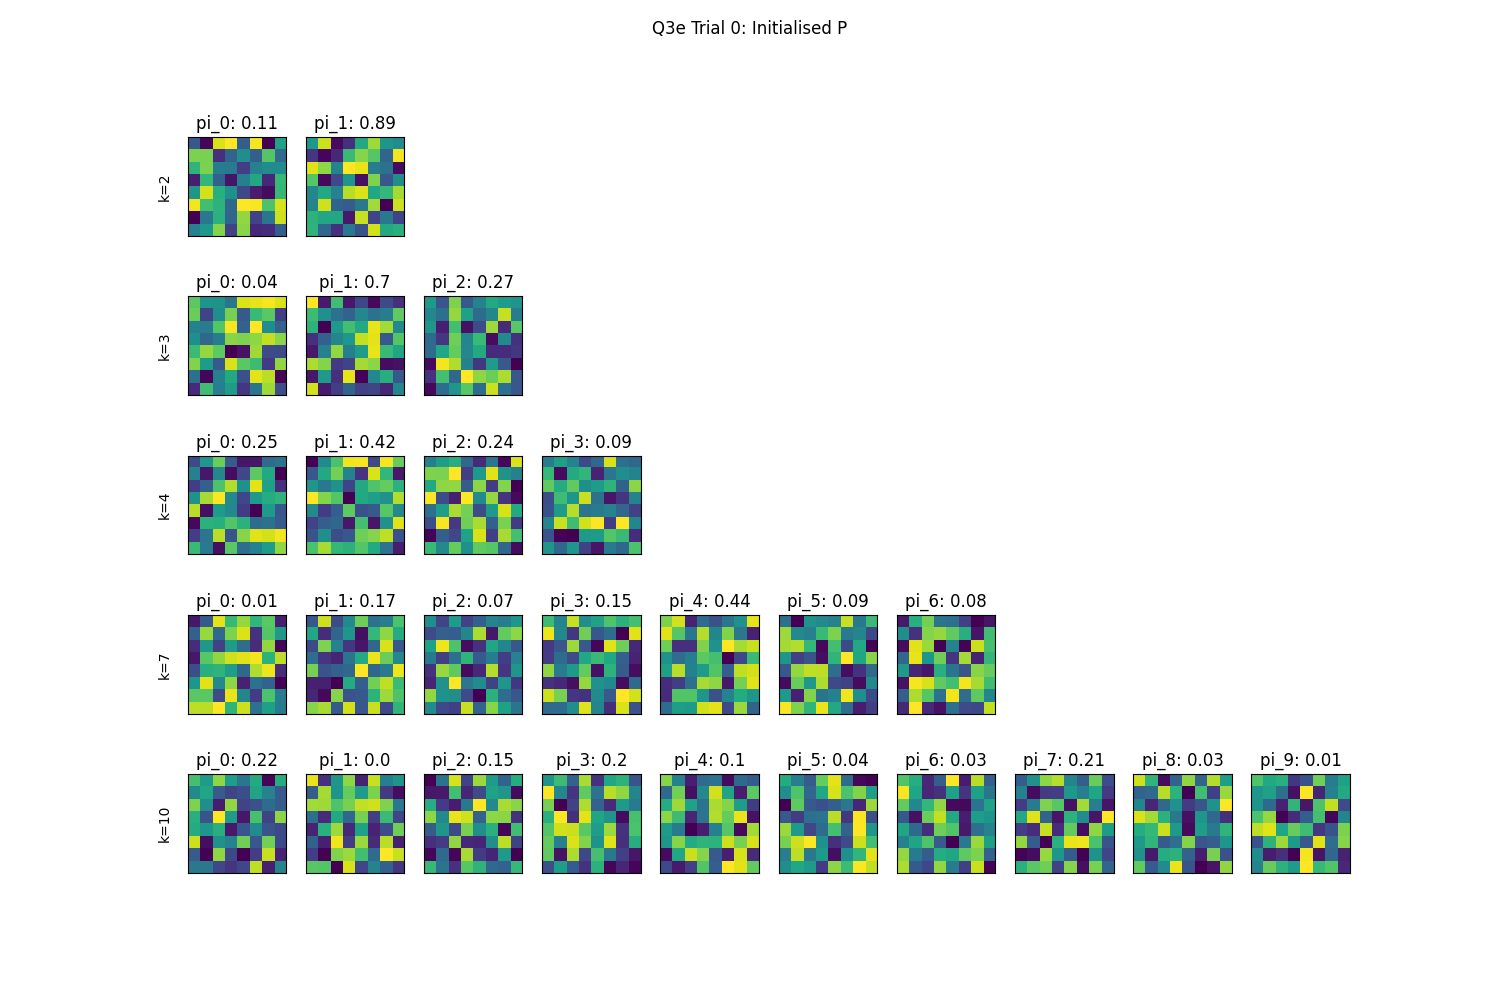
\includegraphics[scale=0.3]{outputs/q3/q3e-0-initialised-p}
  \caption{Randomly initialised parameters}
  \label{fig:3d-initialised-p}
\end{figure}
\begin{figure}[h]
  \centering
  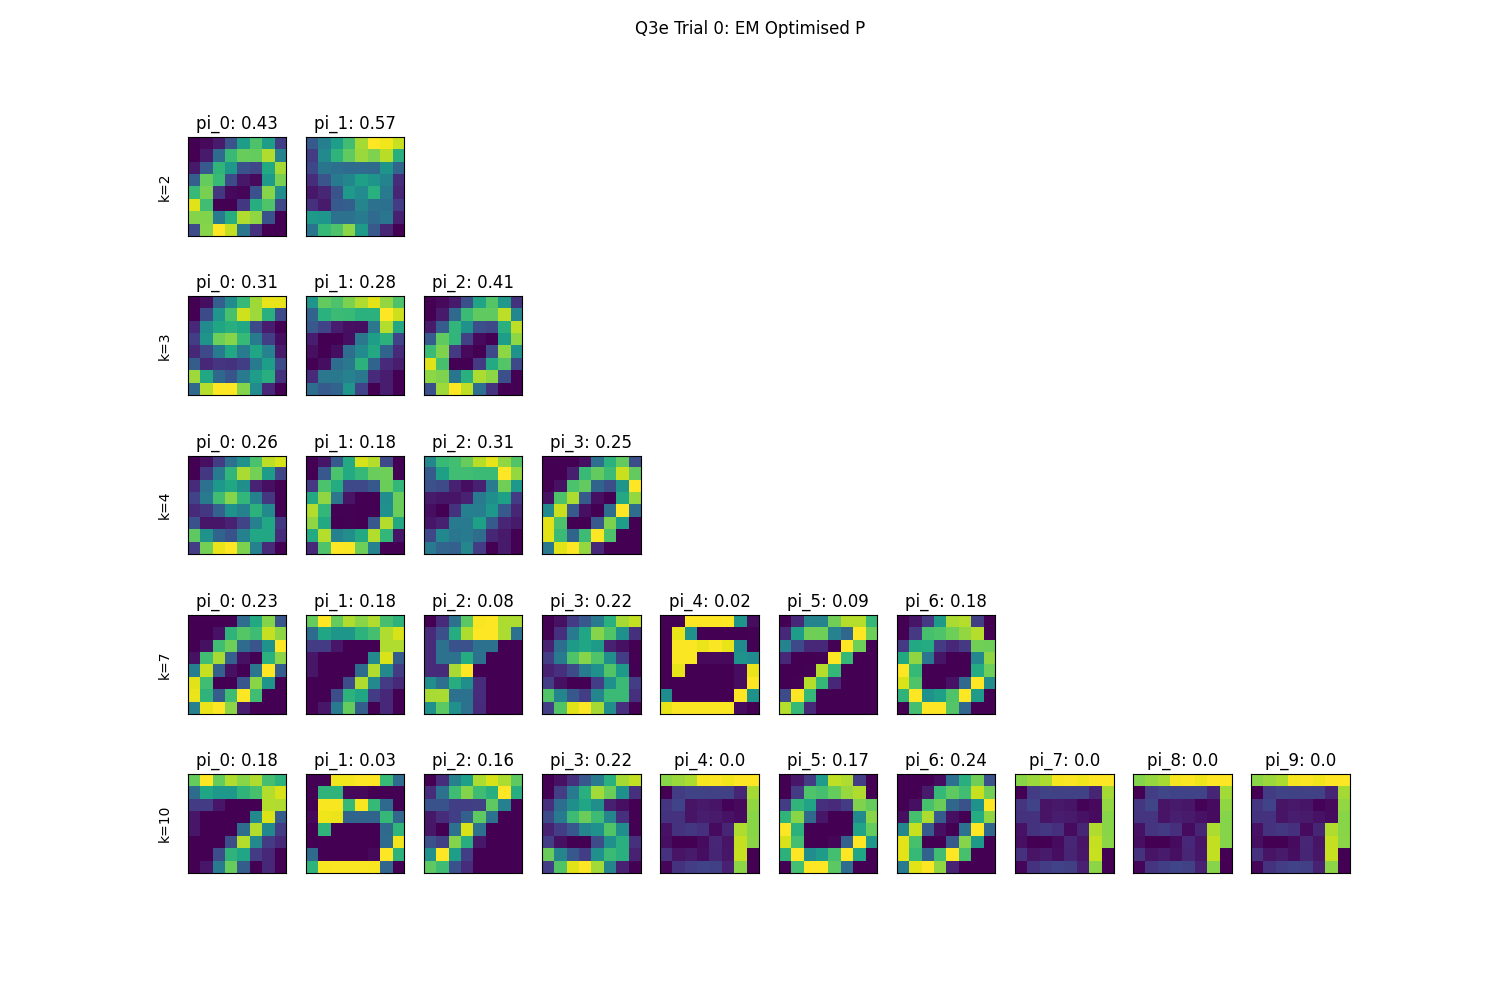
\includegraphics[scale=0.3]{outputs/q3/q3e-0-optimised-p}
  \caption{EM optimised parameters}
  \label{fig:3d-optimised-p}
\end{figure}

\newpage
The Python code for the EM algorithm:
\lstinputlisting[language=Python]{src/solutions/q3.py}
\newpage
\item[(e)] Running the algorithm a few times starting from randomly chosen initial conditions and visualising the parameters:

\begin{figure}[h]
  \centering
  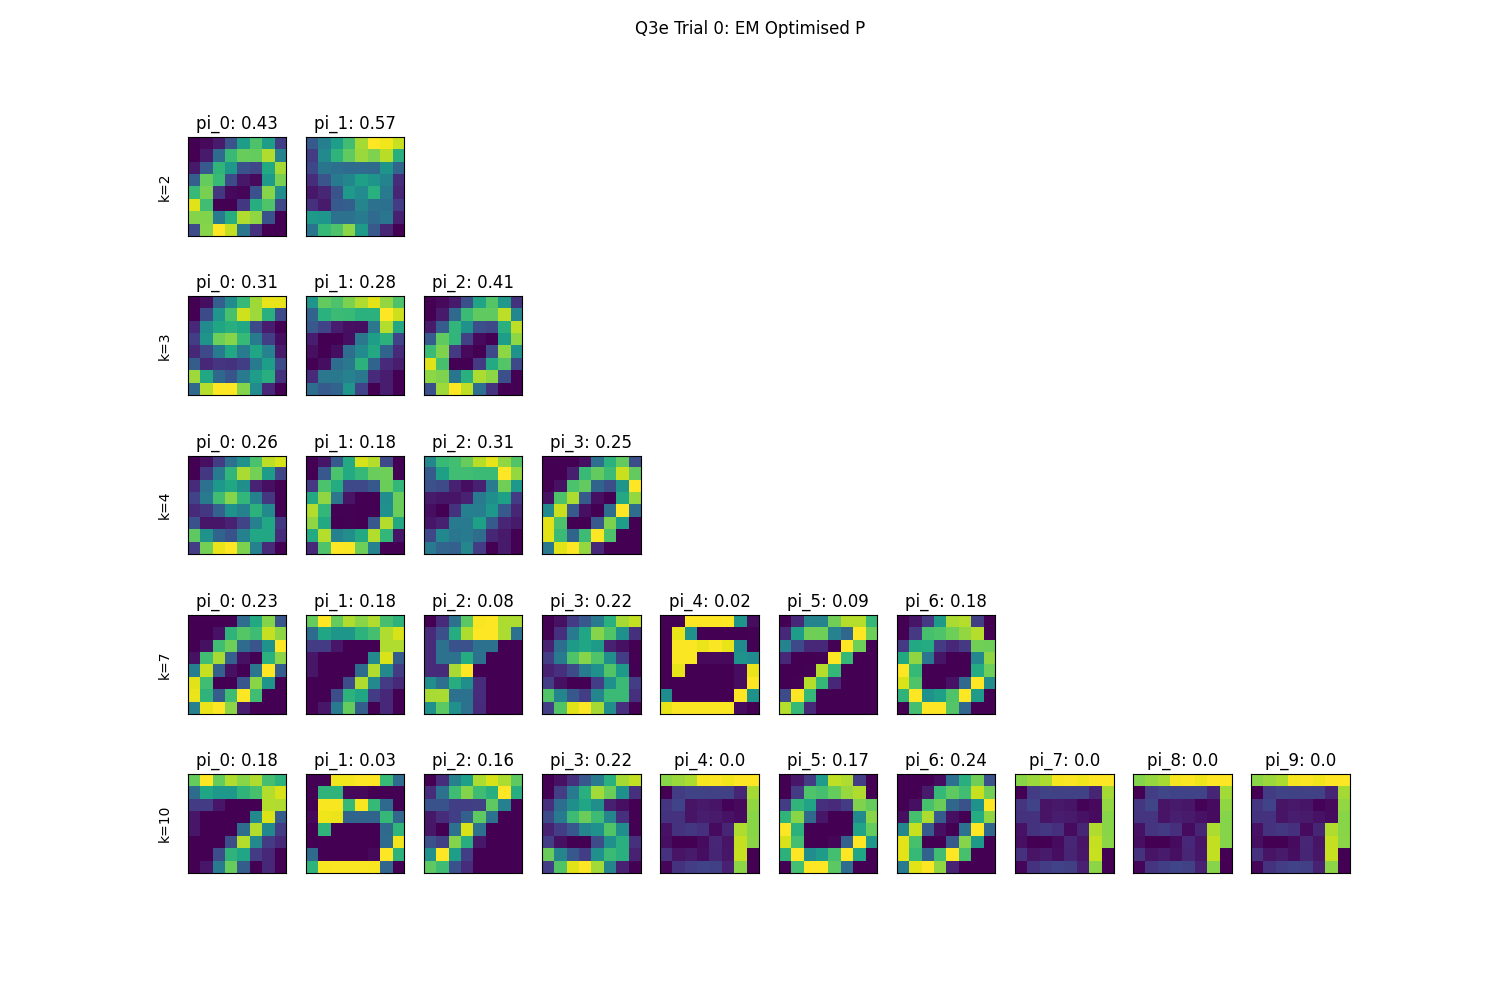
\includegraphics[scale=0.3]{outputs/q3/q3e-0-optimised-p}
  \caption{EM optimised parameters: Trial 0}
  \label{fig:3e-initialised-p-trial-0}
\end{figure}
\begin{figure}[h]
  \centering
  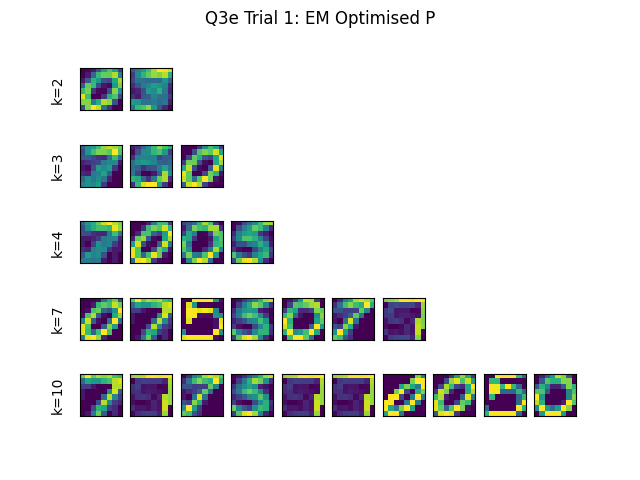
\includegraphics[scale=0.3]{outputs/q3/q3e-1-optimised-p}
  \caption{EM optimised parameters: Trial 1}
  \label{fig:3e-initialised-p-trial-1}
\end{figure}
\newpage

\begin{figure}[h]
  \centering
  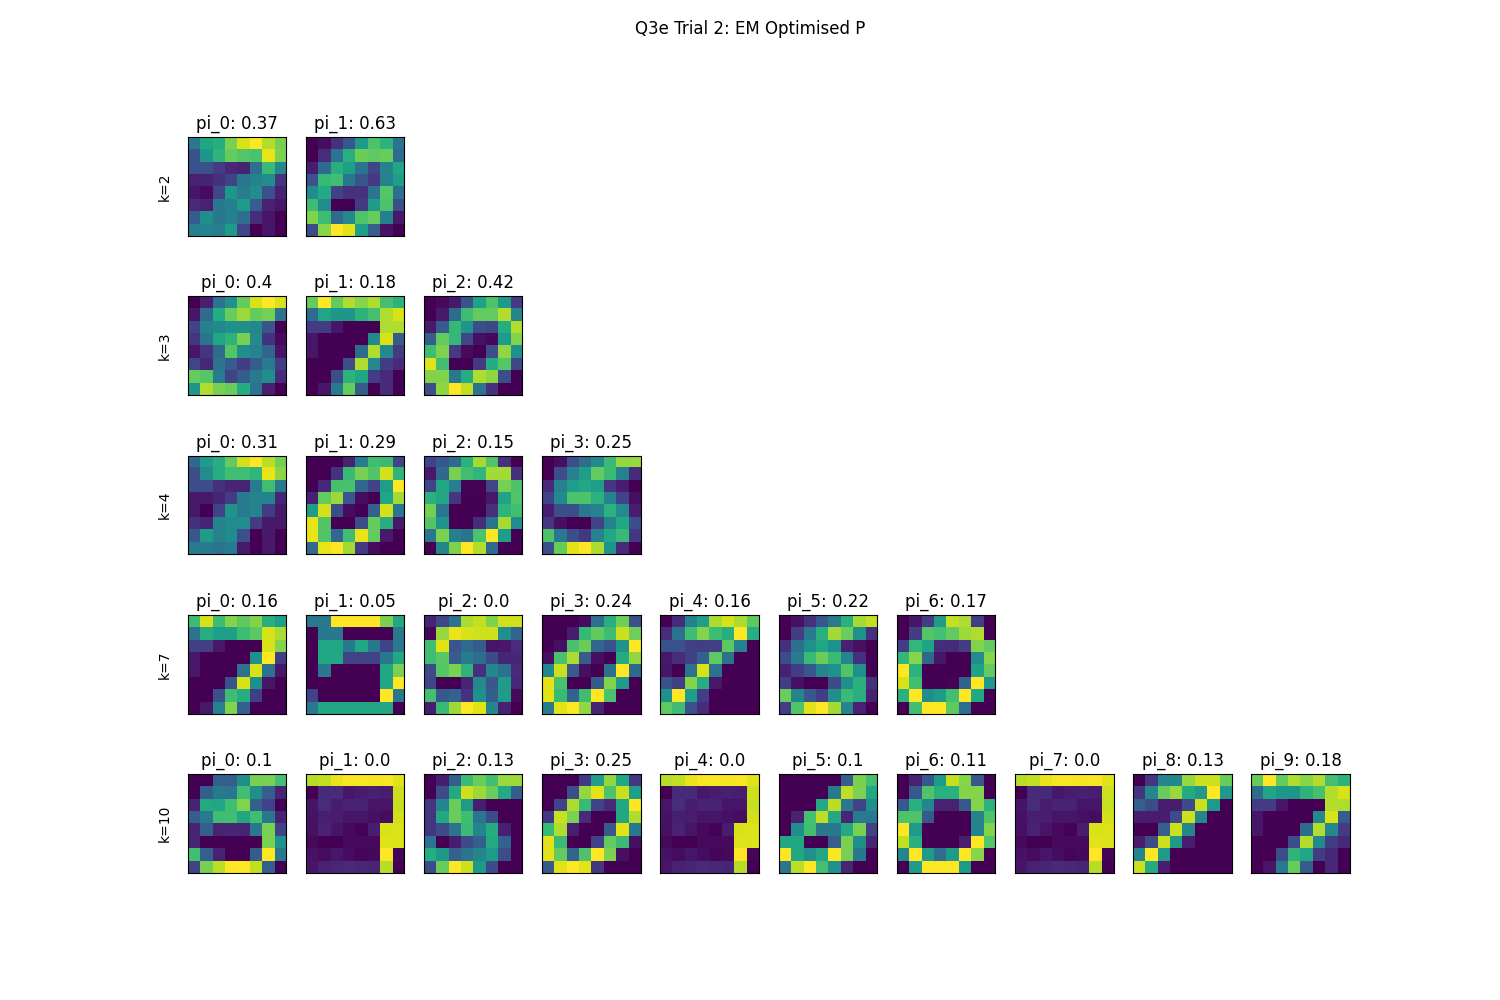
\includegraphics[scale=0.3]{outputs/q3/q3e-2-optimised-p}
  \caption{EM optimised parameters: Trial 2}
  \label{fig:3e-initialised-p-trial-2}
\end{figure}
\begin{figure}[h]
  \centering
  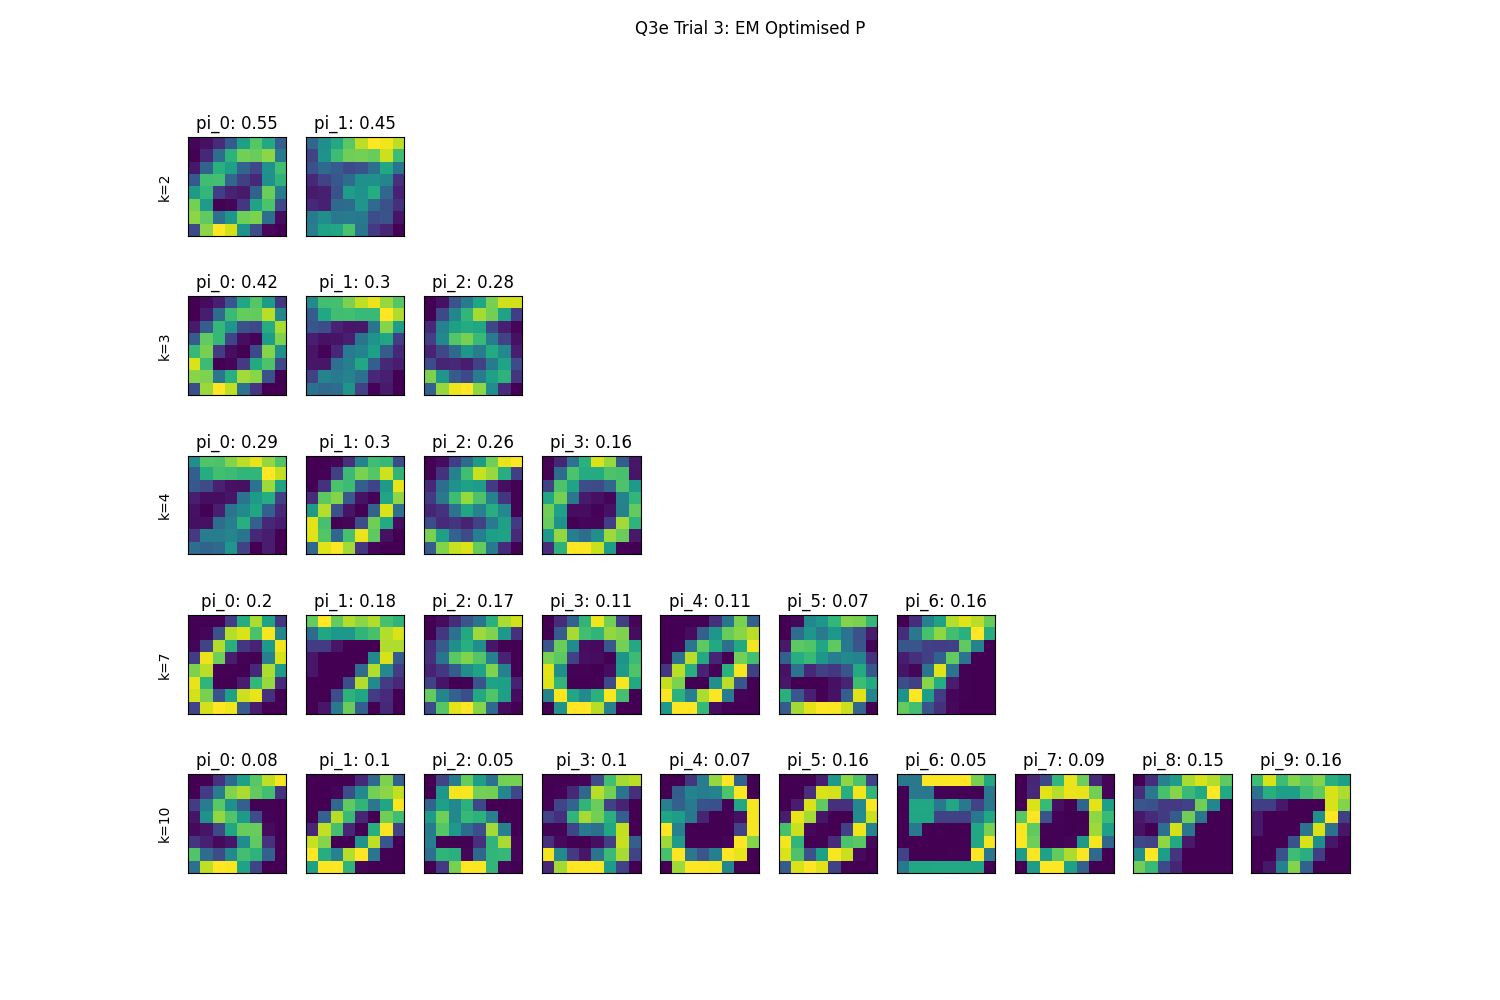
\includegraphics[scale=0.3]{outputs/q3/q3e-3-optimised-p}
  \caption{EM optimised parameters: Trial 3}
  \label{fig:3e-initialised-p-trial-3}
\end{figure}


For smaller k, we can visually see that we obtain very similar solutions (a seven and a zero for $k=2$, although for trial 2, it looks more like zero and five mixed with seven). For $k=3$, we get one each of zero, seven, and five, but in different permutations for different trials. However for higher K, we see that this may not always be the case. For Trial 1 of $k=10$, we have two 5's whereas in Trial 3 we have four 5's. Interestingly, different clusters of the same digits can be different, representing different variants of the written digit (i.e. a slanted zero, a slightly slanted zero, and a symmetric zero).

\newpage

Moreover, looking at the responsibilities of each mixture component, we can see that when k is relatively small they are relatively evenly distributed. However for $k=7$ and especially $k=10$, we can see some components have very small or zero probability (i.e. $\pi_3$ of trial 0 and $k=10$). It will be unlikely for those components to represent very distinct clusters (i.e. the parameters for $\pi_3$ and $\pi_4$ are very similar in trial 0 and $k=10$). Moreover, for these small probabilities, we see that the parameters are almost like binary images. This shows that there are not many images represented in these components. This can be verified when we perform a TSNE visualisation of the responsibility vector for each of the images (Note that for $k=2$, just the responsibility vector is plotted because it is two dimensional). We can see that for large k, qualitatively the number of clusters no longer matches the k value, indicating that some mixtures are redundant. For example for $k=7$ and $k=10$ we can only qualitatively see three or four clusters with TSNE.

\begin{figure}[h]
  \centering
  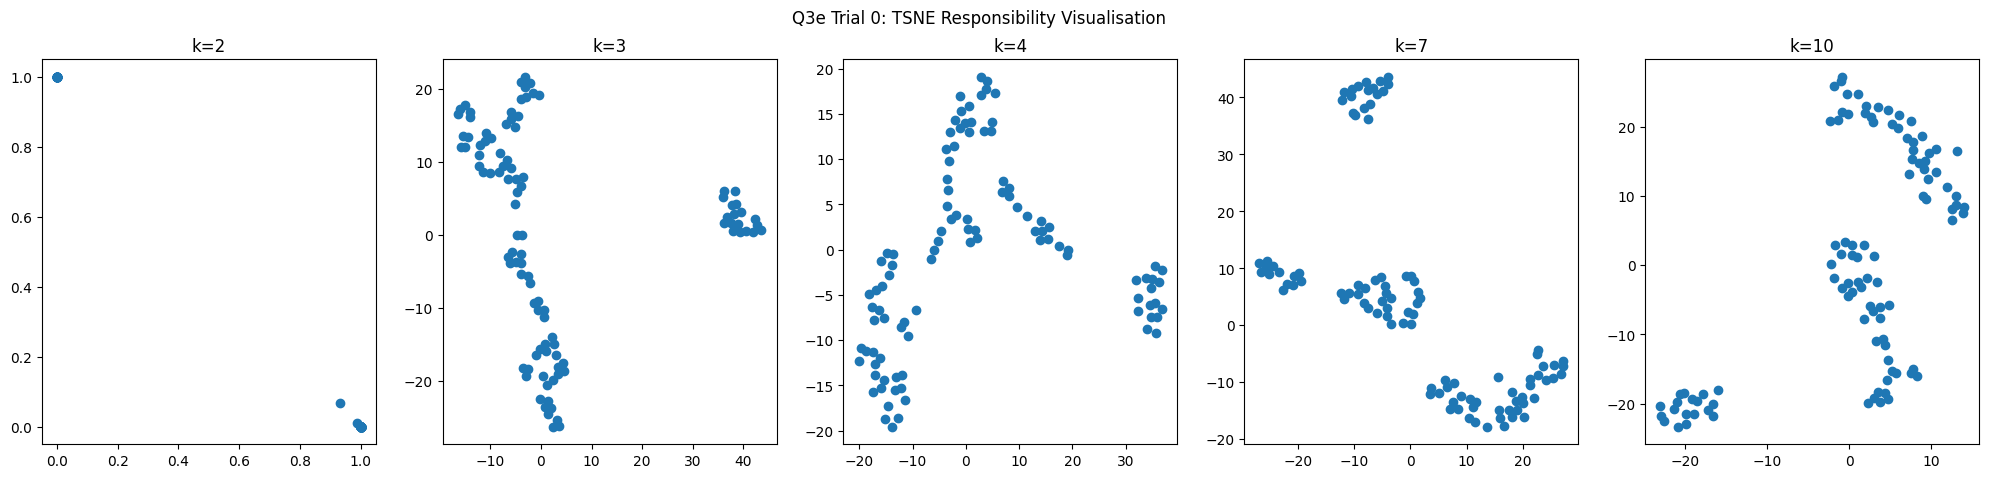
\includegraphics[scale=0.35]{outputs/q3/q3e-0-tsne}
  \caption{TSNE Visualisation of Image responsibilities: Trial 0}
  \label{fig:3e-tsne-0}
\end{figure}
\begin{figure}[h]
  \centering
  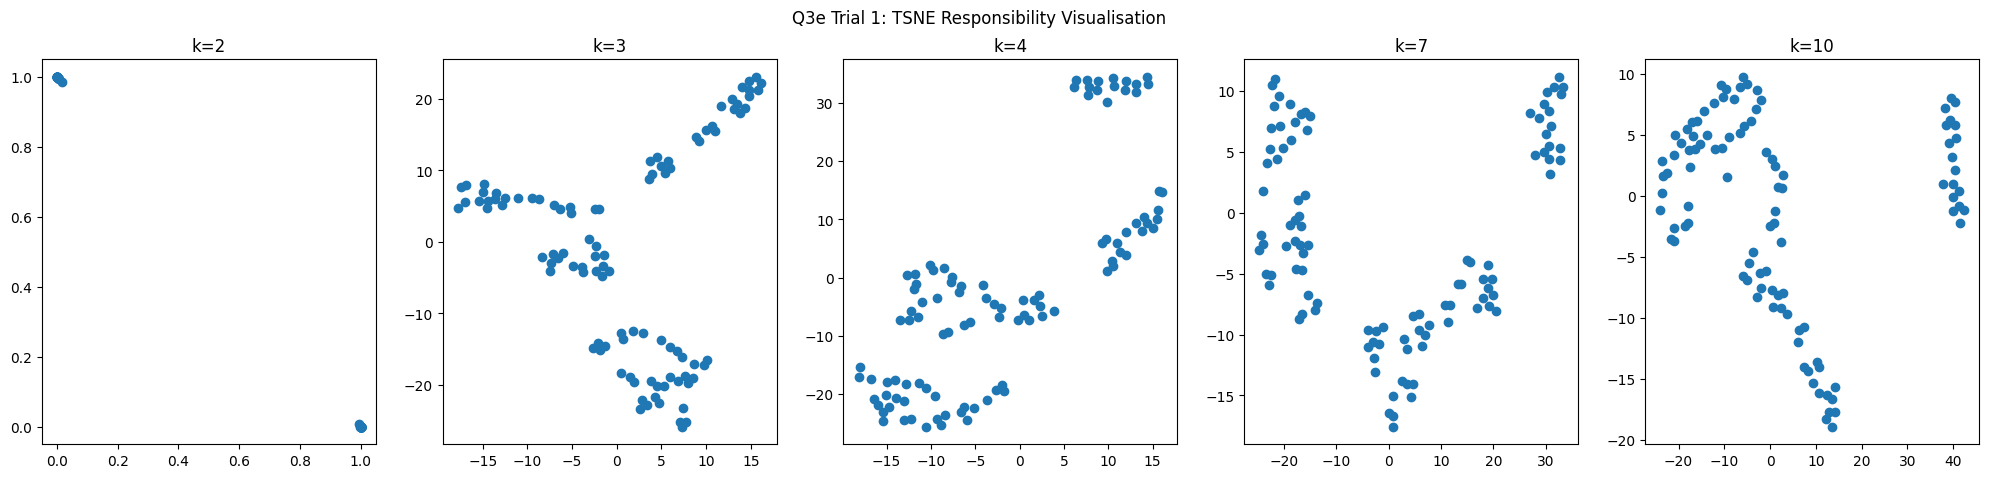
\includegraphics[scale=0.35]{outputs/q3/q3e-1-tsne}
  \caption{TSNE Visualisation of Image responsibilities: Trial 1}
  \label{fig:3e-tsne-1}
\end{figure}
\begin{figure}[h]
  \centering
  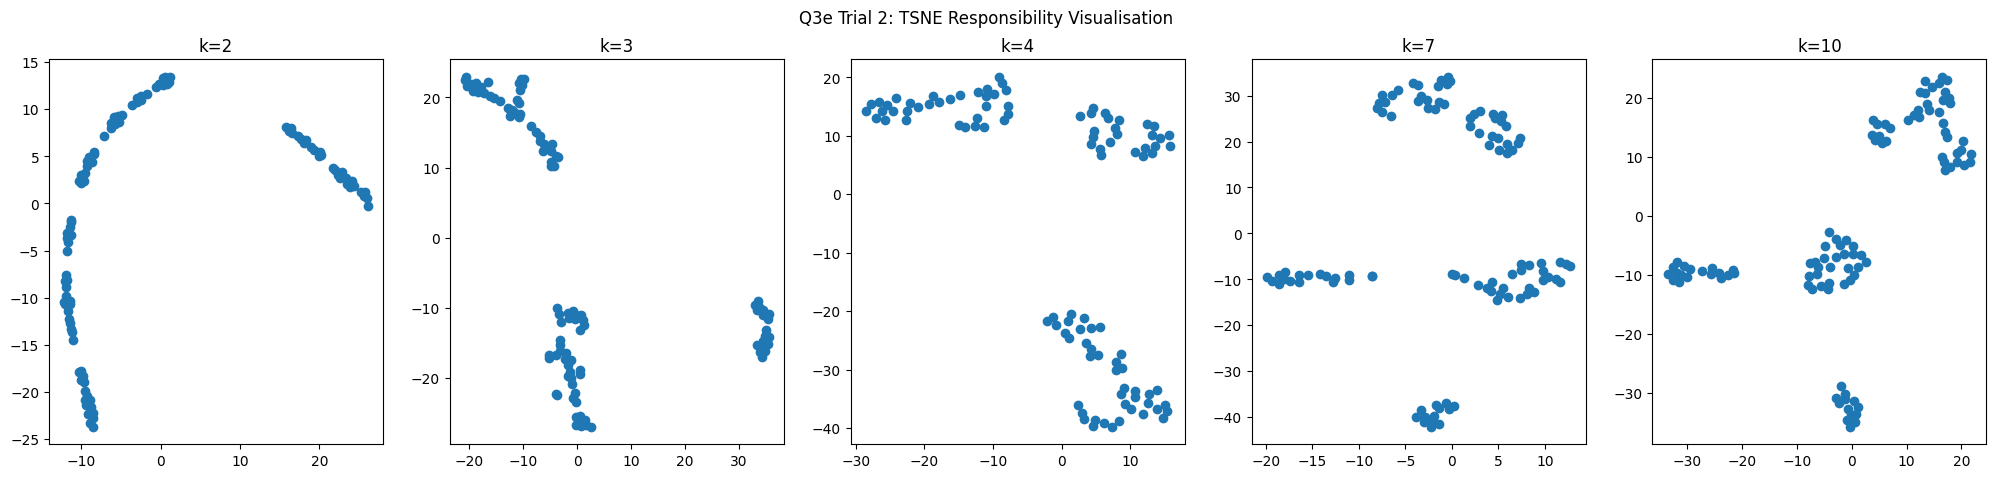
\includegraphics[scale=0.35]{outputs/q3/q3e-2-tsne}
  \caption{TSNE Visualisation of Image responsibilities: Trial 2}
  \label{fig:3e-tsne-2}
\end{figure}
\newpage

\begin{figure}[h]
  \centering
  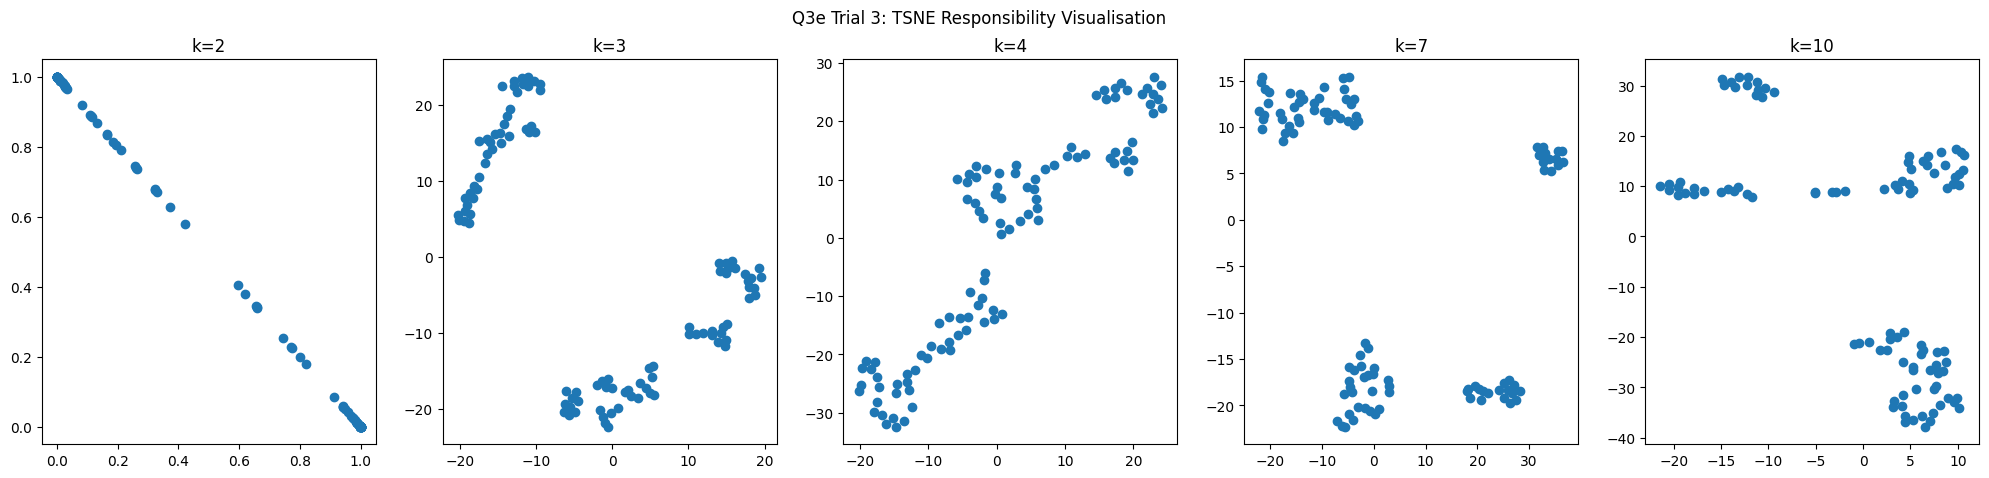
\includegraphics[scale=0.35]{outputs/q3/q3e-3-tsne}
  \caption{TSNE Visualisation of Image responsibilities: Trial 3}
  \label{fig:3e-tsne-3}
\end{figure}

Improvements to the model could include searching for an optimal $k$ by maximising the log posterior with regularisation on the magnitude of $k$ to balance maximising log posterior with minimising model complexity. Additionally, adding a prior on the responsibility components can be helpful to ensure a more even distribution across mixture components unlike the components visualised here. This could help promote more meaningful clusters as $k$ increases.  Moreover, more experimentation for choosing better priors can be helpful to find better separation between mixtures. Finally, increasing the size of our data set (i.e. more images) and resolution of our images (i.e. more pixels) can help the model better understand the distinguishing nuances of different mixtures and provide better clustering, although the number of images and the resolution should scale together to ensure that the model doesn't learn the noise in the higher resolution images. This is assuming we are able to scale our computing resources. Finally, given that we know that there are ten digits and our current data set only includes a subset of these digits, we can also expand our data set to include all ten digits. Hopefully, for $k=10$, we will then be able to achieve a unique digit for each mixing component, rather than variations of repeated digits as we see now.
\newpage
\item[(f)] The log-likelihood in bits can be expressed as:

$$\log_2(P(\{\textbf{x}^{(n)}\}_{n=1}^{N}|\theta))$$

The length of the naive encoding of these binary data is $N \cdot D$, the number of pixels in $\{\textbf{x}^{(n)}\}_{n=1}^{N}$. This is because the images are binary so each pixel can be represented with a single bit. We can compute the ratio of log-likelihood bits to the length of the naive encoding for each $k$:

$$rate = 1 - \frac{\log_2(P(\{\textbf{x}^{(n)}\}_{n=1}^{N}|\theta))}{N \cdot D}$$

Presenting the compression rates for different trials and $k$ values:

\begin{table}[h]
\begin{center}
{\begin{tabular}{c|c|c|c|c}%
 \bfseries k value & Trial 0 & Trial 1& Trial 2 & Trial 3% specify table head
\csvreader[head to column names
]{outputs/q3/q3e-compression.csv}{}% use head of csv as column names
{\\\hline\csvcoli&\csvcolii&\csvcoliii&\csvcoliv&\csvcolv}% specify your coloumns here
\end{tabular}
}
\caption{Compression Rates}
\end{center}
\end{table}

As k increases, we can see that our compression rate gets better. This is intuitive because with higher $k$ we are specifying a more complex and expressive model (i.e. with more parameters) and thus we are able to capture more of the structure of the data in the model. Thus, the bit rate, or information provided by a sample decreases with respect to the complexity of the model and thus our compression rate increases. From the source coding theorem, lossless compression algorithms are lower bounded by the entropy of the underlying data generating distribution $P(\textbf{x})$. This is $-\sum_{x\in \mathcal{X}} P(\textbf{x})\log P(\textbf{x})$. On the other hand, with EM we are maximising $\langle \log P(Z, X | \theta) \rangle_{q(X)} + H[q]$ or minimising the negative of this. When our proposal distribution $P$ matches $q$, we recover $H[P]$ and we get the optimal model, the data generating model for encoding our data, which makes sense because we would be able to compress our data with the best possible distribution. This matches the lower bound of the source coding theorem. However, because it is very unlikely that our proposal $q$ will actually match $P$, our compression rate will always be worse than the optimal compression rate of $H[P]$. On the other hand, a compression algorithm would compressions on a per image basis, independent of the other images. And thus, it is able to attain a better compression rate for that image and is much closer to the source coding theorem lower bound. Depending on the data (i.e. $H[P]$ of the data), the compression rate of gzip can range from $60\%$ to $88\%$ (https://web.dev/optimizing-content-efficiency-optimize-encoding-and-transfer/#text-compression-with-gzip), much higher than that of our models, as we expected.

\newpage
\item[(g)] The total cost of encoding with model parameters and data:

$$\log_2(P(\{\textbf{x}^{(n)}\}_{n=1}^{N}|\theta)) + M \cdot K \cdot D + M \cdot K$$

Where $M$ is the cost of storing a single float value, in our case we used $float64$ so 64 bits. The first term is the log-likelihood as expressed in (f), the second term is the cost of storing $\mathbf{P}$, and the last term is the cost of storing $\pi$. The latter two terms scale with the value of k. This means that as $k$ increases, our compression rate deteriorates. Looking at the total compression ratio $\frac{log_2(P(\{\textbf{x}^{(n)}\}_{n=1}^{N}|\theta)) + M \cdot K \cdot D + M \cdot K}{N\cdot D}$ in a table:

\begin{table}[h]
\begin{center}
{\begin{tabular}{c|c|c|c|c}%
 \bfseries k value & Trial 0 & Trial 1& Trial 2 & Trial 3% specify table head
\csvreader[head to column names
]{outputs/q3/q3e-compression-total.csv}{}% use head of csv as column names
{\\\hline\csvcoli&\csvcolii&\csvcoliii&\csvcoliv&\csvcolv}% specify your coloumns here
\end{tabular}
}
\caption{Total Compression Ratios}
\end{center}
\end{table}

We can see that the ratio is greater than one, meaning that this is actually worse than the naive encoding. This is due to the high cost of each value in the model parameters being 64 bits. However, because this remains constant with respect to our data set size, so as $N$ increases, these ratios will approach $\frac{\log_2(P(\{\textbf{x}^{(n)}\}_{n=1}^{N}|\theta)}{N\cdot D}$ and we'll recover our compression rates from part (f). By increasing $k$, we see that the ratio increases, and thus our compression rate is worse. This makes sense because we are essentially slowly storing the data into the model. In the extreme example of $k=N$ we can have the parameters for each mixture model as an image in the data. Although in this case, we could store our parameters as binary values instead of 64 bit floats. Our mixture component is uniform because each mixture is equally likely (all images are equally likely) so there is no need to store any values for $\pi$. Thus, we would recover the cost of naive encoding our data. Taking into account the model parameters further verifies that the cost of encoding with this approach is much higher than the cost of gzip.


\end{enumerate}



\newpage
\section*{Question 5}

\begin{enumerate}

%\item[] \textbf{[70 points] Decrypting Messages with MCMC.} You are given a passage of English text that has been encrypted by remapping each symbol to a (usually) different one. For example,
%
%$$a \rightarrow s$$
%$$b \rightarrow !$$
%$$\langle space \rangle \rightarrow v$$
%$$\cdots$$
%
%Thus a text like ‘a boy. . . ’ might be encrypted by ‘sv!op. . . ’. Assume that the mapping between symbols is one-to-one. The file symbols.txt gives the list of symbols, one per line (the second line is 〈space〉). The file message.txt gives the encrypted message.
%
%Decoding the message by brute force is impossible, since there are 53 symbols and thus 53! possible permutations to try. Instead we will set up a Markov chain Monte Carlo sampler to find modes in the space of permutations.
%
%We model English text, say $s_1s_2\cdots s_n$ where $s_i$ are symbols, as a Markov chain, so that each symbol is independent of the preceding text given only the symbol before:

%$$p(s_1s_2\cdots s_n) = p(s_1)\prod_{i=2}^{n}p(s_i|s_{i-1})$$

\item[(a)] The formulae for the ML estimates of $P(s_i = \alpha |s_{i-1} = \beta) = \Psi(\alpha, \beta)$:
$$\Psi(\alpha, \beta) = \frac{N_{\alpha, \beta}}{N_{\beta}}$$
where $N_{\alpha, \beta}$ is the count of the number of occurrences of the pair $(\alpha, \beta)$, where $\beta$ is followed by $s\alpha$ in the text and $N_{\beta}$ is the number of occurrences of $\beta$. Moreover to ensure ergodicity, a one was added to each $N_{\alpha, \beta}$. This was also taken into account for the normaliser $N_{\beta}$.

Moreover, the stationary distribution $\phi$ can be calculated using the power method:
\begin{enumerate}
  \item[(i)] Initialise any $\phi^{(0)} \in \mathbb{R}^{53 \times 1}$ and $\sum_i \phi^{(0)}_i = 1$
  \item[(ii)] Repeat $\phi^{(i+1)} = \Psi \phi^{(i)}$
  \item[(iii)] Terminate when $\phi^{(i+1) - \phi^{(i)} < \epsilon$
\end{enumerate}

where $\Psi \in \mathbf{R}^{53\times53}$ containing the transition probabilities, $\Psi_{i, j} = P(s_j | s_i)$ where $s_i$ is the $i^{th}$ symbol and $s_j$ is the $j^{th}$ symbol, and $\epsilon$ is some small number indicating sufficient convergence of the distribution to be considered stationary. The function $\phi(\gamma)$ is simply the index of symbol $\gamma$ in the vector $\phi$.

%Let $p(\textbf{s}_i,\textbf{s}_{i-1})$ be the probability of the pair of symbols $\textbf{s}_i$ and $\textbf{s}_{i-1}$ occurring together in the text ($\textbf{s}_{i-1}$ followed by $\textbf{s}_i$ where order matters).
%We can model $p(\textbf{s}_i,\textbf{s}_{i-1})$ as a multinomial distribution with $N=1$ and $D=53^2$:
%
%$$p(\textbf{s}_i,\textbf{s}_{i-1}) = \frac{1}{s^1! s^2! \cdots s^{53^2}} \prod_{j \in \{1,...53\}, k \in \{1,...53\}} p_{s_i, s_{i-1}}^{t^{s_i, s_{i-1}}}$$
%
%where $t^{s_i, s_{i-1}}$ is an indicator of transition $s_{i-1}$ to $s_i$.
%For convenience we will denote $t^{(\alpha, \beta)})$ as the transition from
%A multinomial distribution is appropriate because there can only be only one of 53 symbols chosen as $s$ (i.e. a 53 dimensional dice).
%Thus, $p(s=s_i)$ represents the probability of the symbol $s_i$ in the text.
%
%We can convert p(s) into exponential family form:
%
%$$p(\textbf{s}) = \frac{1}{s^1! s^2! \cdots s^D} \exp{(\textbf{s}^T \log(\textbf{p}))}$$
%
%where $\textbf{p}$ is the vector of $p_i$'s.
%Thus the sufficient statistic is $T(\textbf{s}) = \textbf{s}^T$.
%
%The ML estimate

%Learn the transition statistics of letters and punctuation in English: Download a large text [say the English translation of War and Peace] from the web and estimate the transition probabilities $p(s_i = \alpha|s_{i-1} = \beta) := \Psi(\alpha, \beta)$, as well as the stationary distribution $\lim_{i\rightarrow \infty} p(s_i = \gamma) := \phi(\gamma)$. Assume that the first letter of your text (and also that of the encrypted text provided) is itself sampled from the stationary distribution. Give formulae for the ML estimates of these probabilities as functions of the counts of numbers of occurrences of symbols and pairs of symbols.
%Compute the estimated probabilities. Report the values as a table. [6 marks]


The transition matrix $\Psi$:


\scalebox{0.18}{
    \centering
    \begin{tabular}{|c|c|c|c|c|c|c|c|c|c|c|c|c|c|c|c|c|c|c|c|c|c|c|c|c|c|c|c|c|c|c|c|c|c|c|c|c|c|c|c|c|c|c|c|c|c|c|c|c|c|c|c|c|c|}
    \hline
        \textbf{} & \textbf{=} & \textbf{space} & \textbf{-} & \textbf{","} & \textbf{;} & \textbf{:} & \textbf{!} & \textbf{?} & \textbf{/} & \textbf{.} & \textbf{'} & \textbf{double quotes} & \textbf{(} & \textbf{)} & \textbf{[} & \textbf{]} & \textbf{*} & \textbf{0} & \textbf{1} & \textbf{2} & \textbf{3} & \textbf{4} & \textbf{5} & \textbf{6} & \textbf{7} & \textbf{8} & \textbf{9} & \textbf{a} & \textbf{b} & \textbf{c} & \textbf{d} & \textbf{e} & \textbf{f} & \textbf{g} & \textbf{h} & \textbf{i} & \textbf{j} & \textbf{k} & \textbf{l} & \textbf{m} & \textbf{n} & \textbf{o} & \textbf{p} & \textbf{q} & \textbf{r} & \textbf{s} & \textbf{t} & \textbf{u} & \textbf{v} & \textbf{w} & \textbf{x} & \textbf{y} & \textbf{z} \\ \hline
        \textbf{=} & 1.8e-02 & 5.9e-06 & 5.3e-04 & 2.5e-05 & 8.4e-04 & 9.4e-04 & 2.5e-04 & 3.2e-04 & 1.6e-02 & 3.2e-05 & 1.7e-02 & 1.3e-02 & 1.4e-03 & 1.4e-03 & 1.8e-02 & 1.8e-02 & 2.9e-03 & 4.5e-03 & 2.3e-03 & 5.1e-03 & 8.9e-03 & 1.3e-02 & 9.8e-03 & 9.4e-03 & 1.1e-02 & 4.1e-03 & 1.2e-02 & 5.0e-06 & 2.9e-05 & 1.6e-05 & 8.5e-06 & 3.2e-06 & 1.8e-05 & 2.0e-05 & 6.0e-06 & 5.9e-06 & 3.9e-04 & 5.0e-05 & 1.1e-05 & 1.6e-05 & 5.5e-06 & 5.3e-06 & 2.2e-05 & 4.2e-04 & 6.8e-06 & 6.4e-06 & 4.5e-06 & 1.6e-05 & 4.0e-05 & 1.7e-05 & 2.3e-04 & 2.2e-05 & 5.5e-04 \\ \hline
        \textbf{space} & 5.5e-02 & 4.2e-03 & 9.0e-03 & 2.5e-05 & 8.4e-04 & 9.4e-04 & 2.5e-04 & 3.2e-04 & 1.6e-02 & 6.5e-04 & 3.3e-02 & 1.5e-01 & 8.1e-01 & 1.4e-03 & 3.6e-02 & 1.8e-02 & 7.9e-01 & 1.3e-02 & 5.1e-01 & 1.2e-01 & 1.3e-01 & 1.3e-01 & 6.9e-02 & 1.7e-01 & 7.7e-02 & 3.7e-02 & 7.1e-02 & 3.1e-01 & 6.6e-01 & 3.1e-01 & 1.3e-01 & 3.3e-02 & 3.5e-01 & 1.7e-01 & 2.7e-01 & 1.6e-01 & 5.7e-01 & 1.8e-01 & 1.3e-01 & 2.9e-01 & 7.3e-02 & 1.7e-01 & 3.6e-01 & 5.4e-01 & 9.2e-02 & 2.4e-01 & 3.6e-01 & 7.9e-02 & 1.4e-01 & 6.3e-01 & 1.0e-01 & 1.3e-01 & 7.0e-02 \\ \hline
        \textbf{-} & 1.8e-02 & 3.3e-05 & 3.2e-03 & 2.5e-05 & 8.4e-04 & 9.4e-04 & 2.5e-04 & 3.2e-04 & 1.6e-02 & 3.2e-05 & 1.7e-02 & 1.3e-02 & 1.4e-03 & 1.4e-03 & 1.8e-02 & 1.8e-02 & 2.9e-03 & 4.5e-03 & 4.5e-03 & 5.1e-03 & 8.9e-03 & 1.3e-02 & 9.8e-03 & 2.8e-02 & 1.1e-02 & 8.2e-03 & 1.2e-02 & 2.5e-04 & 3.4e-03 & 2.9e-03 & 1.3e-03 & 2.5e-04 & 2.4e-03 & 7.1e-04 & 4.4e-04 & 5.3e-04 & 7.7e-04 & 1.8e-03 & 1.3e-03 & 1.1e-03 & 3.7e-04 & 5.0e-04 & 1.2e-03 & 8.5e-04 & 3.7e-04 & 1.1e-03 & 6.0e-04 & 4.8e-04 & 2.8e-04 & 7.6e-04 & 2.3e-04 & 7.3e-04 & 7.1e-03 \\ \hline
        \textbf{","} & 1.8e-02 & 6.7e-02 & 5.3e-04 & 2.5e-05 & 8.4e-04 & 9.4e-04 & 2.5e-04 & 3.2e-04 & 1.6e-02 & 6.5e-05 & 1.7e-02 & 2.7e-02 & 4.2e-03 & 1.4e-03 & 1.8e-02 & 1.8e-02 & 5.9e-03 & 4.5e-02 & 2.3e-03 & 5.1e-03 & 8.9e-03 & 1.3e-02 & 9.8e-03 & 1.9e-02 & 1.1e-02 & 4.1e-03 & 1.2e-02 & 3.0e-03 & 5.8e-03 & 1.9e-03 & 6.5e-04 & 2.3e-04 & 1.5e-03 & 1.2e-03 & 8.6e-04 & 6.4e-04 & 4.6e-03 & 1.0e-03 & 6.3e-04 & 1.1e-03 & 3.4e-04 & 3.8e-04 & 2.4e-03 & 3.4e-03 & 6.2e-04 & 1.3e-03 & 1.1e-03 & 3.4e-04 & 5.5e-04 & 4.7e-03 & 2.3e-04 & 5.3e-04 & 1.1e-03 \\ \hline
        \textbf{;} & 1.8e-02 & 2.1e-03 & 5.3e-04 & 2.5e-05 & 8.4e-04 & 9.4e-04 & 2.5e-04 & 3.2e-04 & 1.6e-02 & 3.2e-05 & 1.7e-02 & 1.3e-02 & 1.4e-03 & 1.4e-03 & 1.8e-02 & 1.8e-02 & 2.9e-03 & 4.5e-03 & 2.3e-03 & 5.1e-03 & 8.9e-03 & 1.3e-02 & 9.8e-03 & 9.4e-03 & 1.1e-02 & 4.1e-03 & 1.2e-02 & 6.0e-05 & 2.6e-04 & 3.3e-05 & 8.5e-06 & 9.6e-06 & 3.7e-05 & 3.9e-05 & 6.6e-05 & 5.3e-05 & 3.9e-04 & 5.0e-05 & 2.1e-05 & 3.3e-05 & 1.1e-05 & 2.6e-05 & 6.6e-05 & 4.2e-04 & 6.8e-06 & 5.1e-05 & 9.4e-05 & 1.6e-05 & 4.0e-05 & 6.9e-05 & 2.3e-04 & 6.6e-05 & 5.5e-04 \\ \hline
        \textbf{:} & 1.8e-02 & 1.5e-03 & 5.3e-04 & 2.5e-05 & 8.4e-04 & 9.4e-04 & 2.5e-04 & 3.2e-04 & 1.6e-02 & 6.5e-05 & 1.7e-02 & 1.3e-02 & 4.2e-03 & 1.4e-03 & 1.8e-02 & 1.8e-02 & 8.8e-03 & 4.5e-03 & 6.8e-03 & 1.0e-02 & 8.9e-03 & 1.3e-02 & 9.8e-03 & 9.4e-03 & 1.1e-02 & 4.1e-03 & 1.2e-02 & 4.0e-05 & 5.9e-05 & 3.3e-05 & 3.4e-05 & 9.6e-06 & 3.7e-05 & 2.0e-05 & 5.4e-05 & 4.1e-05 & 3.9e-04 & 5.0e-05 & 2.1e-05 & 6.5e-05 & 5.5e-06 & 1.6e-05 & 1.1e-04 & 4.2e-04 & 6.8e-06 & 5.1e-05 & 5.8e-05 & 1.6e-05 & 4.0e-05 & 6.9e-05 & 2.3e-04 & 2.2e-05 & 5.5e-04 \\ \hline
        \textbf{!} & 1.8e-02 & 3.0e-03 & 5.3e-04 & 2.5e-05 & 8.4e-04 & 9.4e-04 & 2.5e-04 & 3.2e-04 & 1.6e-02 & 5.7e-03 & 1.7e-02 & 1.3e-02 & 1.4e-03 & 5.7e-03 & 1.8e-02 & 1.8e-02 & 5.9e-03 & 4.5e-03 & 2.3e-03 & 5.1e-03 & 8.9e-03 & 1.3e-02 & 9.8e-03 & 9.4e-03 & 1.1e-02 & 4.1e-03 & 1.2e-02 & 6.5e-05 & 1.2e-04 & 3.3e-05 & 2.5e-05 & 1.3e-05 & 3.7e-05 & 5.9e-05 & 4.2e-05 & 5.3e-05 & 7.7e-04 & 2.5e-04 & 4.2e-05 & 9.8e-05 & 2.8e-05 & 1.6e-05 & 4.4e-05 & 4.2e-04 & 6.8e-06 & 2.6e-05 & 6.3e-05 & 1.6e-05 & 1.2e-04 & 2.3e-04 & 2.3e-04 & 1.3e-04 & 5.5e-04 \\ \hline
        \textbf{?} & 1.8e-02 & 2.3e-03 & 5.3e-04 & 2.5e-05 & 8.4e-04 & 9.4e-04 & 2.5e-04 & 3.2e-04 & 1.6e-02 & 3.8e-03 & 1.7e-02 & 1.3e-02 & 4.2e-03 & 4.3e-03 & 1.8e-02 & 1.8e-02 & 2.9e-03 & 4.5e-03 & 2.3e-03 & 5.1e-03 & 8.9e-03 & 1.3e-02 & 9.8e-03 & 9.4e-03 & 1.1e-02 & 4.1e-03 & 1.2e-02 & 3.0e-05 & 1.8e-04 & 4.9e-05 & 3.4e-05 & 9.6e-06 & 5.5e-05 & 2.0e-05 & 8.4e-05 & 1.1e-04 & 3.9e-04 & 5.0e-05 & 2.1e-05 & 3.3e-05 & 4.4e-05 & 2.1e-05 & 4.4e-05 & 4.2e-04 & 6.8e-06 & 1.9e-05 & 7.6e-05 & 1.6e-05 & 4.0e-05 & 2.9e-04 & 2.3e-04 & 1.1e-04 & 5.5e-04 \\ \hline
        \textbf{/} & 1.8e-02 & 2.0e-06 & 5.3e-04 & 2.5e-05 & 8.4e-04 & 9.4e-04 & 2.5e-04 & 3.2e-04 & 1.6e-02 & 3.2e-05 & 1.7e-02 & 1.3e-02 & 1.4e-03 & 1.4e-03 & 1.8e-02 & 1.8e-02 & 2.9e-03 & 4.5e-03 & 2.3e-03 & 5.1e-03 & 8.9e-03 & 2.6e-02 & 9.8e-03 & 9.4e-03 & 1.1e-02 & 4.1e-03 & 1.2e-02 & 5.0e-06 & 2.9e-05 & 4.9e-05 & 2.5e-05 & 3.2e-06 & 1.8e-05 & 2.0e-05 & 1.2e-05 & 5.9e-06 & 3.9e-04 & 5.0e-05 & 2.1e-05 & 1.6e-05 & 5.5e-06 & 5.3e-06 & 2.2e-05 & 4.2e-04 & 6.8e-06 & 6.4e-06 & 9.0e-06 & 1.6e-05 & 4.0e-05 & 1.7e-05 & 2.3e-04 & 4.4e-05 & 5.5e-04 \\ \hline
        \textbf{.} & 1.8e-02 & 2.9e-02 & 5.3e-04 & 2.3e-04 & 8.4e-04 & 9.4e-04 & 3.0e-03 & 5.4e-03 & 1.6e-02 & 1.3e-01 & 1.7e-02 & 2.7e-02 & 2.4e-02 & 1.0e-01 & 1.8e-02 & 1.8e-02 & 1.5e-02 & 4.5e-03 & 5.9e-02 & 2.0e-02 & 7.1e-02 & 3.9e-02 & 2.9e-02 & 2.8e-02 & 5.5e-02 & 2.1e-02 & 4.8e-02 & 3.2e-03 & 9.4e-03 & 6.0e-03 & 1.1e-03 & 2.7e-04 & 2.3e-03 & 5.7e-04 & 2.3e-03 & 2.0e-03 & 1.4e-02 & 2.6e-03 & 4.3e-04 & 1.3e-03 & 1.5e-03 & 1.2e-03 & 8.8e-03 & 1.7e-03 & 6.4e-04 & 1.9e-03 & 5.2e-03 & 1.7e-04 & 2.4e-04 & 5.2e-03 & 2.3e-04 & 5.5e-04 & 3.8e-03 \\ \hline
        \textbf{'} & 1.8e-02 & 2.0e-06 & 5.3e-04 & 5.0e-05 & 8.4e-04 & 9.4e-04 & 2.5e-04 & 3.2e-04 & 1.6e-02 & 3.2e-05 & 1.7e-02 & 1.3e-02 & 1.4e-03 & 1.4e-03 & 1.8e-02 & 1.8e-02 & 2.9e-03 & 4.5e-03 & 2.3e-03 & 5.1e-03 & 8.9e-03 & 1.3e-02 & 9.8e-03 & 9.4e-03 & 1.1e-02 & 4.1e-03 & 1.2e-02 & 9.9e-06 & 2.9e-05 & 1.6e-05 & 8.5e-06 & 3.2e-06 & 1.8e-05 & 2.0e-05 & 6.0e-06 & 5.9e-06 & 3.9e-04 & 5.0e-05 & 1.1e-05 & 1.6e-05 & 5.5e-06 & 5.3e-06 & 2.2e-05 & 4.2e-04 & 6.8e-06 & 3.9e-05 & 4.5e-06 & 1.6e-05 & 4.0e-05 & 1.7e-05 & 2.3e-04 & 2.2e-05 & 5.5e-04 \\ \hline
        \textbf{double quotes} & 1.8e-02 & 2.0e-05 & 5.3e-04 & 2.5e-05 & 8.4e-04 & 9.4e-04 & 2.5e-04 & 3.2e-04 & 1.6e-02 & 3.2e-05 & 1.7e-02 & 1.3e-02 & 1.4e-03 & 2.9e-03 & 1.8e-02 & 1.8e-02 & 5.9e-03 & 4.5e-03 & 2.3e-03 & 5.1e-03 & 8.9e-03 & 1.3e-02 & 9.8e-03 & 9.4e-03 & 1.1e-02 & 4.1e-03 & 1.2e-02 & 5.0e-06 & 2.9e-05 & 1.6e-05 & 1.7e-05 & 3.2e-06 & 1.8e-05 & 2.0e-05 & 6.0e-06 & 1.2e-05 & 3.9e-04 & 5.0e-05 & 1.1e-05 & 1.6e-05 & 5.5e-06 & 5.3e-06 & 1.8e-04 & 4.2e-04 & 1.4e-05 & 6.4e-06 & 9.0e-06 & 1.6e-05 & 4.0e-05 & 1.7e-05 & 2.3e-04 & 2.2e-05 & 5.5e-04 \\ \hline
        \textbf{(} & 1.8e-02 & 2.0e-06 & 5.3e-04 & 2.5e-05 & 8.4e-04 & 9.4e-04 & 2.5e-04 & 3.2e-04 & 1.6e-02 & 3.2e-05 & 1.7e-02 & 2.7e-02 & 1.4e-03 & 1.4e-03 & 1.8e-02 & 1.8e-02 & 2.9e-03 & 4.5e-03 & 4.1e-02 & 2.0e-01 & 1.4e-01 & 5.3e-02 & 2.0e-02 & 9.4e-03 & 1.1e-02 & 8.2e-03 & 1.2e-02 & 4.1e-04 & 5.0e-04 & 9.8e-05 & 6.8e-05 & 2.6e-05 & 2.7e-04 & 9.8e-05 & 4.6e-04 & 2.6e-04 & 7.7e-04 & 3.0e-04 & 7.4e-05 & 2.1e-04 & 9.9e-05 & 1.8e-04 & 5.3e-04 & 8.5e-04 & 3.4e-05 & 2.9e-04 & 4.5e-04 & 4.7e-05 & 1.6e-04 & 1.4e-03 & 2.3e-04 & 4.4e-05 & 5.5e-04 \\ \hline
        \textbf{)} & 1.8e-02 & 7.8e-04 & 5.3e-04 & 4.3e-03 & 5.1e-03 & 1.9e-03 & 2.5e-04 & 3.2e-04 & 1.6e-02 & 1.2e-03 & 1.7e-02 & 1.3e-02 & 2.8e-03 & 1.4e-03 & 1.8e-02 & 1.8e-02 & 2.9e-03 & 4.5e-03 & 2.3e-03 & 5.1e-03 & 8.9e-03 & 1.3e-02 & 9.8e-03 & 9.4e-03 & 1.1e-02 & 4.1e-03 & 1.2e-02 & 4.0e-05 & 8.8e-05 & 1.6e-05 & 8.5e-06 & 3.2e-06 & 3.7e-05 & 2.0e-05 & 1.8e-05 & 2.3e-05 & 3.9e-04 & 5.0e-05 & 1.1e-05 & 3.3e-05 & 5.5e-06 & 2.1e-05 & 6.6e-05 & 4.2e-04 & 6.8e-06 & 1.3e-05 & 3.6e-05 & 1.6e-05 & 4.0e-05 & 6.9e-05 & 2.3e-04 & 2.2e-05 & 5.5e-04 \\ \hline
        \textbf{[} & 1.8e-02 & 2.0e-06 & 5.3e-04 & 2.5e-05 & 8.4e-04 & 9.4e-04 & 2.5e-04 & 3.2e-04 & 1.6e-02 & 3.2e-05 & 1.7e-02 & 1.3e-02 & 1.4e-03 & 1.4e-03 & 1.8e-02 & 1.8e-02 & 2.9e-03 & 4.5e-03 & 2.3e-03 & 5.1e-03 & 8.9e-03 & 1.3e-02 & 9.8e-03 & 9.4e-03 & 1.1e-02 & 4.1e-03 & 1.2e-02 & 5.0e-06 & 2.9e-05 & 1.6e-05 & 8.5e-06 & 6.4e-06 & 1.8e-05 & 2.0e-05 & 6.0e-06 & 5.9e-06 & 3.9e-04 & 5.0e-05 & 1.1e-05 & 3.3e-05 & 5.5e-06 & 5.3e-06 & 2.2e-05 & 4.2e-04 & 6.8e-06 & 6.4e-06 & 4.5e-06 & 1.6e-05 & 4.0e-05 & 1.7e-05 & 2.3e-04 & 2.2e-05 & 5.5e-04 \\ \hline
        \textbf{]} & 1.8e-02 & 2.0e-06 & 5.3e-04 & 2.5e-05 & 8.4e-04 & 9.4e-04 & 2.5e-04 & 3.2e-04 & 1.6e-02 & 3.2e-05 & 1.7e-02 & 1.3e-02 & 1.4e-03 & 1.4e-03 & 3.6e-02 & 1.8e-02 & 2.9e-03 & 4.5e-03 & 2.3e-03 & 5.1e-03 & 8.9e-03 & 1.3e-02 & 9.8e-03 & 9.4e-03 & 1.1e-02 & 4.1e-03 & 1.2e-02 & 5.0e-06 & 2.9e-05 & 1.6e-05 & 8.5e-06 & 3.2e-06 & 1.8e-05 & 2.0e-05 & 6.0e-06 & 5.9e-06 & 3.9e-04 & 5.0e-05 & 2.1e-05 & 1.6e-05 & 5.5e-06 & 5.3e-06 & 2.2e-05 & 4.2e-04 & 6.8e-06 & 6.4e-06 & 4.5e-06 & 1.6e-05 & 4.0e-05 & 1.7e-05 & 2.3e-04 & 2.2e-05 & 5.5e-04 \\ \hline
        \textbf{*} & 1.8e-02 & 4.9e-04 & 5.3e-04 & 2.5e-05 & 8.4e-04 & 9.4e-04 & 2.5e-04 & 3.2e-04 & 1.6e-02 & 3.2e-05 & 1.7e-02 & 1.3e-02 & 2.4e-02 & 1.4e-03 & 1.8e-02 & 1.8e-02 & 2.6e-02 & 4.5e-03 & 2.3e-03 & 5.1e-03 & 8.9e-03 & 1.3e-02 & 9.8e-03 & 9.4e-03 & 1.1e-02 & 4.1e-03 & 1.2e-02 & 1.5e-05 & 2.9e-05 & 3.3e-05 & 1.7e-05 & 3.2e-06 & 1.8e-05 & 2.0e-05 & 6.0e-06 & 1.2e-05 & 3.9e-04 & 1.0e-04 & 1.1e-05 & 1.6e-05 & 5.5e-06 & 5.3e-06 & 4.4e-05 & 4.2e-04 & 6.8e-06 & 6.4e-06 & 4.5e-06 & 3.1e-05 & 4.0e-05 & 5.2e-05 & 2.3e-04 & 4.4e-05 & 5.5e-04 \\ \hline
        \textbf{0} & 1.8e-02 & 8.2e-05 & 5.3e-04 & 3.0e-04 & 8.4e-04 & 9.4e-04 & 2.5e-04 & 3.2e-04 & 1.6e-02 & 6.5e-05 & 1.7e-02 & 1.3e-02 & 1.4e-03 & 2.9e-03 & 1.8e-02 & 3.6e-02 & 2.9e-03 & 1.3e-01 & 1.1e-02 & 2.0e-02 & 8.9e-03 & 1.3e-02 & 2.7e-01 & 1.2e-01 & 1.8e-01 & 2.5e-02 & 2.1e-01 & 5.0e-06 & 2.9e-05 & 4.9e-05 & 8.5e-06 & 3.2e-06 & 1.8e-05 & 2.0e-05 & 6.0e-06 & 5.9e-06 & 3.9e-04 & 5.0e-05 & 1.1e-05 & 1.6e-05 & 5.5e-06 & 5.3e-06 & 2.2e-05 & 4.2e-04 & 6.8e-06 & 6.4e-06 & 4.5e-06 & 1.6e-05 & 4.0e-05 & 3.5e-05 & 2.3e-04 & 2.2e-05 & 5.5e-04 \\ \hline
        \textbf{1} & 1.8e-02 & 3.5e-05 & 5.3e-04 & 1.3e-04 & 8.4e-04 & 9.4e-04 & 2.5e-04 & 3.2e-04 & 1.6e-02 & 1.6e-03 & 1.7e-02 & 1.3e-02 & 2.8e-03 & 2.7e-02 & 1.8e-02 & 1.8e-02 & 2.9e-03 & 7.2e-02 & 3.8e-02 & 3.2e-01 & 1.9e-01 & 3.9e-02 & 9.8e-02 & 3.8e-02 & 9.9e-02 & 6.9e-01 & 1.2e-02 & 5.0e-06 & 2.9e-05 & 3.3e-05 & 8.5e-06 & 3.2e-06 & 1.8e-05 & 2.0e-05 & 6.0e-06 & 5.9e-06 & 3.9e-04 & 5.0e-05 & 1.1e-05 & 1.6e-05 & 5.5e-06 & 5.3e-06 & 2.2e-05 & 4.2e-04 & 6.8e-06 & 1.3e-05 & 4.5e-06 & 1.6e-05 & 4.0e-05 & 1.7e-05 & 2.3e-04 & 2.2e-05 & 5.5e-04 \\ \hline
        \textbf{2} & 1.8e-02 & 6.7e-05 & 5.3e-04 & 3.5e-04 & 8.4e-04 & 9.4e-04 & 2.5e-04 & 6.3e-04 & 1.6e-02 & 4.5e-04 & 1.7e-02 & 1.3e-02 & 1.4e-03 & 5.7e-02 & 1.8e-02 & 3.6e-02 & 2.9e-03 & 5.8e-02 & 6.8e-03 & 3.1e-02 & 2.7e-02 & 5.3e-02 & 3.9e-02 & 2.8e-02 & 3.3e-02 & 4.1e-03 & 1.2e-02 & 9.9e-06 & 2.9e-05 & 1.3e-04 & 8.5e-06 & 3.2e-06 & 1.8e-05 & 2.0e-05 & 6.0e-06 & 5.9e-06 & 3.9e-04 & 1.0e-04 & 1.1e-05 & 1.6e-05 & 1.1e-05 & 5.3e-06 & 2.2e-05 & 4.2e-04 & 6.8e-06 & 6.4e-06 & 4.5e-06 & 1.6e-05 & 4.0e-05 & 1.7e-05 & 2.3e-04 & 2.2e-05 & 5.5e-04 \\ \hline
        \textbf{3} & 1.8e-02 & 2.5e-05 & 5.3e-04 & 1.8e-04 & 8.4e-04 & 9.4e-04 & 2.5e-04 & 3.2e-04 & 1.6e-02 & 2.6e-04 & 1.7e-02 & 1.3e-02 & 1.4e-03 & 2.4e-02 & 1.8e-02 & 1.8e-02 & 2.9e-03 & 3.6e-02 & 4.5e-03 & 5.1e-03 & 8.9e-03 & 1.3e-02 & 9.8e-03 & 9.4e-03 & 1.1e-02 & 4.1e-03 & 1.2e-02 & 5.0e-06 & 2.9e-05 & 3.3e-05 & 8.5e-06 & 3.2e-06 & 1.8e-05 & 2.0e-05 & 6.0e-06 & 5.9e-06 & 3.9e-04 & 5.0e-05 & 1.1e-05 & 1.6e-05 & 5.5e-06 & 5.3e-06 & 2.2e-05 & 4.2e-04 & 4.1e-05 & 6.4e-06 & 1.8e-05 & 1.6e-05 & 4.0e-05 & 1.7e-05 & 2.3e-04 & 2.2e-05 & 5.5e-04 \\ \hline
        \textbf{4} & 1.8e-02 & 9.8e-06 & 1.1e-03 & 7.5e-05 & 8.4e-04 & 9.4e-04 & 2.5e-04 & 3.2e-04 & 1.6e-02 & 2.3e-04 & 1.7e-02 & 1.3e-02 & 1.4e-03 & 5.7e-03 & 1.8e-02 & 1.8e-02 & 2.9e-03 & 1.3e-02 & 6.8e-03 & 5.1e-03 & 8.9e-03 & 1.3e-02 & 9.8e-03 & 9.4e-03 & 1.1e-02 & 4.1e-03 & 1.2e-02 & 5.0e-06 & 2.9e-05 & 1.6e-05 & 8.5e-06 & 3.2e-06 & 1.8e-05 & 2.0e-05 & 6.0e-06 & 5.9e-06 & 3.9e-04 & 5.0e-05 & 1.1e-05 & 1.6e-05 & 5.5e-06 & 5.3e-06 & 2.2e-05 & 4.2e-04 & 6.8e-06 & 6.4e-06 & 1.3e-05 & 1.6e-05 & 4.0e-05 & 1.7e-05 & 4.5e-04 & 2.2e-05 & 5.5e-04 \\ \hline
        \textbf{5} & 1.8e-02 & 1.8e-05 & 1.1e-03 & 4.3e-04 & 1.7e-03 & 1.9e-03 & 2.5e-04 & 3.2e-04 & 3.2e-02 & 2.9e-04 & 1.7e-02 & 1.3e-02 & 1.4e-03 & 2.9e-03 & 1.8e-02 & 1.8e-02 & 2.9e-03 & 3.1e-02 & 2.3e-03 & 5.1e-03 & 8.9e-03 & 2.6e-02 & 9.8e-03 & 9.4e-03 & 1.1e-02 & 4.1e-03 & 2.4e-02 & 5.0e-06 & 2.9e-05 & 6.5e-05 & 8.5e-06 & 3.2e-06 & 1.8e-05 & 2.0e-05 & 6.0e-06 & 5.9e-06 & 3.9e-04 & 5.0e-05 & 1.1e-05 & 1.6e-05 & 5.5e-06 & 5.3e-06 & 2.2e-05 & 4.2e-04 & 6.8e-06 & 6.4e-06 & 9.0e-06 & 1.6e-05 & 4.0e-05 & 1.7e-05 & 2.3e-04 & 4.4e-05 & 5.5e-04 \\ \hline
        \textbf{6} & 1.8e-02 & 2.2e-05 & 1.6e-03 & 2.3e-04 & 1.7e-03 & 9.4e-04 & 2.5e-04 & 6.3e-04 & 1.6e-02 & 1.9e-04 & 1.7e-02 & 1.3e-02 & 1.4e-03 & 1.4e-03 & 1.8e-02 & 1.8e-02 & 2.9e-03 & 2.7e-02 & 2.3e-03 & 1.5e-02 & 8.9e-03 & 2.6e-02 & 9.8e-03 & 1.2e-01 & 2.2e-02 & 4.1e-03 & 1.2e-02 & 5.0e-06 & 2.9e-05 & 3.3e-05 & 8.5e-06 & 3.2e-06 & 1.8e-05 & 2.0e-05 & 6.0e-06 & 5.9e-06 & 3.9e-04 & 5.0e-05 & 1.1e-05 & 1.6e-05 & 5.5e-06 & 5.3e-06 & 2.2e-05 & 4.2e-04 & 6.8e-06 & 6.4e-06 & 1.8e-05 & 1.6e-05 & 4.0e-05 & 1.7e-05 & 2.3e-04 & 2.2e-05 & 5.5e-04 \\ \hline
        \textbf{7} & 1.8e-02 & 2.7e-05 & 5.3e-04 & 2.0e-04 & 8.4e-04 & 9.4e-04 & 5.0e-04 & 3.2e-04 & 1.6e-02 & 1.6e-04 & 1.7e-02 & 1.3e-02 & 1.4e-03 & 1.4e-03 & 1.8e-02 & 1.8e-02 & 2.9e-03 & 1.8e-02 & 4.5e-03 & 5.1e-03 & 8.9e-03 & 1.3e-02 & 9.8e-03 & 9.4e-03 & 1.1e-02 & 2.1e-02 & 2.4e-02 & 5.0e-06 & 2.9e-05 & 3.3e-05 & 8.5e-06 & 3.2e-06 & 1.8e-05 & 2.0e-05 & 6.0e-06 & 5.9e-06 & 3.9e-04 & 5.0e-05 & 1.1e-05 & 1.6e-05 & 5.5e-06 & 5.3e-06 & 2.2e-05 & 4.2e-04 & 6.8e-06 & 6.4e-06 & 1.8e-05 & 1.6e-05 & 4.0e-05 & 1.7e-05 & 2.3e-04 & 2.2e-05 & 5.5e-04 \\ \hline
        \textbf{8} & 1.8e-02 & 1.6e-05 & 5.3e-04 & 7.5e-05 & 8.4e-04 & 9.4e-04 & 2.5e-04 & 3.2e-04 & 1.6e-02 & 1.6e-04 & 1.7e-02 & 1.3e-02 & 1.4e-03 & 1.4e-03 & 1.8e-02 & 1.8e-02 & 2.9e-03 & 3.6e-01 & 1.9e-01 & 2.6e-02 & 8.9e-03 & 2.6e-02 & 9.8e-03 & 1.9e-02 & 2.2e-02 & 8.2e-03 & 4.8e-02 & 5.0e-06 & 2.9e-05 & 1.6e-05 & 8.5e-06 & 3.2e-06 & 1.8e-05 & 2.0e-05 & 6.0e-06 & 5.9e-06 & 3.9e-04 & 5.0e-05 & 1.1e-05 & 1.6e-05 & 5.5e-06 & 1.1e-05 & 4.4e-05 & 4.2e-04 & 6.8e-06 & 6.4e-06 & 1.3e-05 & 1.6e-05 & 4.0e-05 & 1.7e-05 & 2.3e-04 & 2.2e-05 & 5.5e-04 \\ \hline
        \textbf{9} & 1.8e-02 & 2.7e-05 & 5.3e-04 & 1.5e-04 & 8.4e-04 & 1.9e-03 & 2.5e-04 & 3.2e-04 & 1.6e-02 & 1.9e-04 & 1.7e-02 & 1.3e-02 & 1.4e-03 & 1.4e-03 & 1.8e-02 & 1.8e-02 & 2.9e-03 & 1.8e-02 & 2.3e-03 & 5.1e-03 & 8.9e-03 & 1.3e-02 & 9.8e-03 & 1.9e-02 & 2.2e-02 & 4.1e-03 & 1.2e-02 & 5.0e-06 & 5.9e-05 & 1.6e-05 & 8.5e-06 & 3.2e-06 & 1.8e-05 & 2.0e-05 & 6.0e-06 & 5.9e-06 & 3.9e-04 & 5.0e-05 & 1.1e-05 & 1.6e-05 & 5.5e-06 & 5.3e-06 & 2.2e-05 & 4.2e-04 & 6.8e-06 & 6.4e-06 & 9.0e-06 & 1.6e-05 & 4.0e-05 & 1.7e-05 & 2.3e-04 & 2.2e-05 & 5.5e-04 \\ \hline
        \textbf{a} & 1.8e-02 & 2.4e-02 & 2.0e-02 & 2.4e-02 & 1.7e-02 & 6.6e-03 & 3.3e-02 & 1.7e-02 & 1.6e-02 & 1.6e-02 & 1.7e-02 & 1.3e-02 & 4.2e-03 & 1.4e-02 & 1.8e-02 & 1.8e-02 & 2.9e-03 & 4.5e-03 & 2.3e-03 & 5.1e-03 & 8.9e-03 & 1.3e-02 & 9.8e-03 & 9.4e-03 & 1.1e-02 & 4.1e-03 & 1.2e-02 & 1.3e-04 & 1.0e-01 & 1.2e-01 & 9.6e-02 & 2.4e-04 & 3.1e-02 & 6.7e-02 & 2.1e-03 & 5.1e-02 & 6.8e-02 & 1.3e-01 & 1.5e-01 & 7.7e-02 & 2.5e-01 & 2.5e-04 & 1.0e-01 & 3.8e-03 & 1.2e-01 & 1.3e-01 & 1.3e-01 & 3.9e-02 & 1.7e-01 & 3.8e-02 & 1.2e-02 & 1.2e-01 & 1.9e-01 \\ \hline
        \textbf{b} & 1.8e-02 & 2.2e-04 & 3.2e-03 & 9.0e-04 & 8.4e-04 & 9.4e-04 & 5.0e-04 & 9.5e-04 & 1.6e-02 & 6.5e-04 & 1.7e-02 & 1.3e-02 & 1.4e-03 & 4.3e-03 & 1.8e-02 & 1.8e-02 & 2.9e-03 & 4.5e-03 & 2.3e-03 & 5.1e-03 & 8.9e-03 & 1.3e-02 & 9.8e-03 & 9.4e-03 & 1.1e-02 & 4.1e-03 & 1.2e-02 & 1.6e-02 & 6.8e-03 & 6.5e-05 & 1.6e-04 & 3.6e-02 & 1.8e-05 & 2.0e-05 & 1.8e-05 & 5.9e-03 & 6.8e-02 & 5.0e-05 & 3.8e-02 & 1.1e-03 & 5.0e-05 & 2.2e-02 & 2.2e-05 & 4.2e-04 & 1.3e-02 & 3.1e-03 & 1.2e-03 & 8.2e-02 & 1.9e-03 & 3.8e-04 & 2.3e-04 & 5.7e-02 & 5.5e-04 \\ \hline
        \textbf{c} & 1.8e-02 & 9.2e-04 & 1.6e-03 & 9.8e-04 & 3.4e-03 & 1.9e-03 & 1.0e-03 & 6.3e-04 & 1.6e-02 & 1.0e-03 & 1.7e-02 & 1.3e-02 & 1.4e-03 & 5.7e-03 & 1.8e-02 & 1.8e-02 & 2.9e-03 & 4.5e-03 & 2.3e-03 & 5.1e-03 & 8.9e-03 & 1.3e-02 & 9.8e-03 & 9.4e-03 & 1.1e-02 & 4.1e-03 & 1.2e-02 & 3.3e-02 & 8.8e-05 & 1.7e-02 & 9.3e-05 & 4.2e-02 & 7.3e-05 & 9.8e-05 & 7.0e-02 & 1.5e-02 & 3.9e-04 & 1.3e-01 & 2.1e-02 & 9.8e-05 & 1.1e-05 & 6.8e-02 & 6.6e-05 & 5.0e-02 & 1.4e-02 & 6.8e-04 & 1.9e-02 & 2.6e-02 & 4.0e-05 & 1.7e-04 & 2.3e-04 & 6.9e-03 & 3.3e-03 \\ \hline
        \textbf{d} & 1.8e-02 & 1.2e-01 & 1.2e-01 & 1.1e-01 & 1.0e-01 & 1.8e-01 & 8.0e-02 & 5.9e-02 & 1.6e-02 & 9.1e-02 & 1.7e-02 & 2.7e-02 & 7.1e-03 & 6.8e-02 & 1.8e-02 & 1.8e-02 & 2.9e-03 & 4.5e-03 & 2.3e-03 & 5.1e-03 & 8.9e-03 & 1.3e-02 & 9.8e-03 & 9.4e-03 & 1.1e-02 & 4.1e-03 & 1.2e-02 & 1.5e-02 & 9.1e-03 & 3.3e-03 & 1.3e-02 & 4.4e-02 & 4.6e-03 & 1.0e-02 & 2.7e-03 & 4.7e-02 & 1.0e-01 & 5.1e-03 & 1.4e-02 & 7.9e-03 & 2.9e-03 & 2.7e-02 & 5.0e-03 & 2.6e-02 & 2.5e-02 & 1.7e-02 & 3.7e-03 & 1.8e-02 & 1.4e-02 & 5.2e-03 & 2.3e-04 & 2.7e-02 & 3.3e-03 \\ \hline
        \textbf{e} & 1.8e-02 & 1.8e-01 & 1.5e-01 & 1.5e-01 & 1.3e-01 & 1.5e-01 & 1.7e-01 & 1.8e-01 & 1.6e-02 & 1.4e-01 & 3.3e-02 & 1.3e-02 & 8.5e-03 & 1.1e-01 & 1.8e-02 & 1.8e-02 & 2.9e-03 & 4.5e-03 & 2.3e-03 & 1.0e-02 & 8.9e-03 & 1.3e-02 & 9.8e-03 & 9.4e-03 & 1.1e-02 & 4.1e-03 & 1.2e-02 & 7.0e-02 & 1.7e-02 & 9.6e-02 & 2.5e-01 & 2.6e-02 & 6.5e-02 & 4.5e-02 & 7.2e-03 & 2.2e-02 & 3.8e-02 & 1.6e-02 & 1.1e-01 & 1.2e-01 & 1.5e-01 & 1.1e-02 & 8.4e-02 & 1.3e-01 & 3.0e-01 & 1.3e-01 & 3.6e-02 & 6.2e-03 & 2.1e-01 & 6.5e-02 & 7.1e-01 & 8.3e-02 & 9.5e-02 \\ \hline
        \textbf{f} & 1.8e-02 & 3.3e-02 & 9.0e-02 & 1.2e-02 & 8.4e-03 & 1.9e-02 & 1.3e-02 & 9.8e-03 & 1.6e-02 & 1.4e-02 & 1.7e-02 & 1.3e-02 & 2.8e-03 & 1.9e-02 & 1.8e-02 & 1.8e-02 & 2.9e-03 & 4.5e-03 & 1.1e-02 & 5.1e-03 & 8.9e-03 & 1.3e-02 & 9.8e-03 & 9.4e-03 & 1.1e-02 & 4.1e-03 & 1.2e-02 & 2.0e-02 & 2.2e-03 & 9.1e-04 & 2.4e-04 & 1.5e-02 & 5.2e-02 & 5.9e-04 & 9.1e-04 & 2.8e-02 & 2.3e-03 & 8.5e-04 & 1.3e-02 & 9.2e-04 & 1.3e-04 & 4.3e-02 & 1.1e-03 & 1.3e-03 & 3.9e-02 & 1.4e-03 & 1.1e-02 & 2.9e-02 & 5.9e-04 & 1.5e-03 & 2.3e-04 & 2.3e-03 & 5.5e-04 \\ \hline
        \textbf{g} & 1.8e-02 & 3.5e-02 & 5.5e-02 & 3.7e-02 & 3.7e-02 & 5.8e-02 & 3.5e-02 & 4.4e-02 & 8.1e-02 & 3.4e-02 & 1.7e-02 & 8.0e-02 & 1.4e-03 & 3.1e-02 & 1.8e-02 & 1.8e-02 & 2.9e-03 & 4.5e-03 & 2.3e-03 & 5.1e-03 & 8.9e-03 & 1.3e-02 & 9.8e-03 & 9.4e-03 & 1.1e-02 & 4.1e-03 & 1.2e-02 & 1.8e-02 & 1.8e-03 & 6.7e-04 & 7.1e-04 & 1.9e-02 & 1.1e-03 & 9.1e-03 & 3.7e-02 & 1.5e-02 & 2.3e-03 & 1.5e-04 & 1.6e-02 & 9.6e-04 & 5.3e-03 & 1.7e-02 & 1.1e-03 & 8.5e-04 & 1.9e-02 & 6.1e-03 & 2.0e-03 & 2.1e-02 & 5.1e-04 & 1.8e-03 & 2.3e-04 & 2.2e-03 & 1.6e-03 \\ \hline
        \textbf{h} & 1.8e-02 & 2.4e-02 & 2.0e-02 & 3.2e-02 & 2.6e-02 & 1.4e-02 & 5.0e-02 & 3.5e-02 & 1.6e-02 & 1.8e-02 & 1.7e-02 & 1.3e-02 & 5.6e-03 & 1.7e-02 & 1.8e-02 & 1.8e-02 & 2.9e-03 & 4.5e-03 & 4.5e-03 & 5.1e-03 & 8.9e-03 & 1.3e-02 & 9.8e-03 & 9.4e-03 & 1.1e-02 & 4.1e-03 & 1.2e-02 & 1.4e-01 & 2.6e-03 & 1.7e-03 & 8.5e-04 & 2.4e-01 & 1.7e-03 & 4.7e-04 & 7.3e-04 & 1.5e-01 & 7.7e-04 & 5.0e-03 & 1.7e-03 & 6.7e-03 & 7.8e-04 & 7.2e-02 & 1.1e-03 & 4.2e-04 & 8.9e-03 & 1.5e-03 & 2.0e-02 & 2.5e-02 & 5.1e-04 & 1.8e-03 & 2.3e-04 & 2.0e-02 & 5.5e-04 \\ \hline
        \textbf{i} & 1.8e-02 & 8.9e-03 & 1.2e-02 & 5.6e-03 & 3.4e-03 & 1.9e-03 & 5.5e-03 & 1.4e-02 & 1.6e-02 & 4.2e-03 & 1.7e-02 & 4.0e-02 & 2.8e-03 & 1.4e-03 & 1.8e-02 & 1.8e-02 & 2.9e-03 & 4.5e-03 & 2.3e-03 & 5.1e-03 & 8.9e-03 & 1.3e-02 & 9.8e-03 & 9.4e-03 & 1.1e-02 & 4.1e-03 & 1.2e-02 & 1.5e-02 & 3.8e-02 & 1.4e-01 & 7.4e-02 & 2.7e-02 & 6.9e-02 & 8.4e-02 & 2.4e-04 & 2.9e-03 & 3.9e-04 & 6.0e-02 & 8.4e-02 & 1.6e-01 & 2.7e-01 & 3.8e-02 & 1.9e-02 & 1.2e-02 & 4.0e-02 & 1.4e-01 & 9.5e-02 & 2.1e-03 & 1.4e-01 & 8.7e-04 & 7.3e-02 & 4.4e-05 & 3.2e-01 \\ \hline
        \textbf{j} & 1.8e-02 & 2.0e-06 & 5.3e-04 & 2.5e-05 & 8.4e-04 & 9.4e-04 & 2.5e-04 & 3.2e-04 & 1.6e-02 & 3.2e-05 & 1.7e-02 & 1.3e-02 & 1.4e-03 & 1.4e-03 & 1.8e-02 & 1.8e-02 & 2.9e-03 & 4.5e-03 & 2.3e-03 & 5.1e-03 & 8.9e-03 & 1.3e-02 & 9.8e-03 & 9.4e-03 & 1.1e-02 & 4.1e-03 & 1.2e-02 & 4.8e-04 & 2.9e-05 & 1.6e-05 & 8.5e-06 & 1.8e-03 & 1.8e-05 & 2.0e-05 & 6.0e-06 & 7.0e-05 & 3.9e-04 & 5.0e-05 & 1.1e-05 & 1.6e-05 & 5.5e-06 & 3.8e-03 & 2.2e-05 & 4.2e-04 & 6.8e-06 & 6.4e-06 & 4.5e-06 & 1.8e-02 & 4.0e-05 & 1.7e-05 & 2.3e-04 & 2.2e-05 & 5.5e-04 \\ \hline
        \textbf{k} & 1.8e-02 & 7.3e-03 & 1.8e-02 & 1.4e-02 & 1.4e-02 & 1.0e-02 & 1.6e-02 & 1.7e-02 & 3.2e-02 & 1.3e-02 & 1.7e-02 & 1.3e-02 & 2.8e-03 & 1.0e-02 & 1.8e-02 & 1.8e-02 & 2.9e-03 & 4.5e-03 & 2.3e-03 & 5.1e-03 & 8.9e-03 & 1.3e-02 & 9.8e-03 & 9.4e-03 & 1.1e-02 & 4.1e-03 & 1.2e-02 & 2.7e-03 & 5.3e-04 & 9.3e-04 & 6.8e-05 & 1.8e-02 & 4.7e-04 & 2.7e-04 & 5.0e-03 & 2.0e-02 & 7.7e-04 & 5.0e-05 & 3.6e-03 & 6.0e-04 & 1.1e-02 & 1.5e-03 & 2.4e-04 & 4.2e-04 & 6.8e-04 & 4.9e-03 & 2.0e-04 & 1.0e-02 & 5.5e-04 & 1.7e-03 & 2.3e-04 & 2.3e-03 & 5.5e-04 \\ \hline
        \textbf{l} & 1.8e-02 & 1.9e-02 & 6.0e-02 & 3.5e-02 & 2.9e-02 & 2.1e-02 & 3.6e-02 & 2.3e-02 & 1.6e-02 & 2.0e-02 & 1.7e-02 & 1.3e-02 & 2.8e-03 & 2.0e-02 & 1.8e-02 & 1.8e-02 & 2.9e-03 & 4.5e-03 & 2.3e-03 & 5.1e-03 & 8.9e-03 & 1.3e-02 & 9.8e-03 & 9.4e-03 & 1.1e-02 & 4.1e-03 & 1.2e-02 & 3.8e-02 & 3.0e-03 & 1.8e-03 & 5.9e-02 & 5.4e-02 & 4.3e-02 & 2.1e-03 & 3.2e-04 & 5.5e-02 & 3.9e-04 & 5.2e-02 & 1.4e-01 & 7.0e-03 & 7.5e-04 & 4.4e-02 & 9.3e-03 & 2.5e-03 & 3.4e-03 & 1.1e-02 & 7.9e-03 & 2.3e-02 & 1.7e-02 & 8.8e-03 & 2.3e-04 & 2.2e-01 & 1.4e-02 \\ \hline
        \textbf{m} & 1.8e-02 & 1.7e-02 & 4.3e-03 & 3.6e-02 & 5.4e-02 & 4.3e-02 & 3.0e-02 & 3.3e-02 & 1.6e-02 & 5.3e-02 & 3.3e-02 & 1.3e-02 & 1.4e-03 & 3.9e-02 & 1.8e-02 & 1.8e-02 & 2.9e-03 & 4.5e-03 & 2.3e-03 & 5.1e-03 & 8.9e-03 & 1.3e-02 & 9.8e-03 & 9.4e-03 & 1.1e-02 & 4.1e-03 & 1.2e-02 & 4.6e-02 & 3.3e-02 & 9.0e-04 & 8.5e-05 & 4.8e-02 & 2.9e-03 & 2.4e-04 & 3.2e-04 & 2.8e-02 & 1.5e-03 & 5.0e-04 & 1.8e-03 & 2.3e-02 & 1.3e-03 & 3.5e-02 & 7.7e-02 & 4.2e-04 & 6.4e-04 & 1.3e-02 & 8.7e-04 & 2.6e-02 & 2.4e-04 & 9.2e-04 & 2.3e-04 & 5.4e-02 & 5.5e-04 \\ \hline
        \textbf{n} & 1.8e-02 & 6.4e-02 & 8.3e-02 & 7.6e-02 & 7.6e-02 & 6.6e-02 & 6.6e-02 & 6.3e-02 & 1.6e-02 & 6.5e-02 & 6.7e-02 & 2.7e-02 & 5.6e-03 & 5.7e-02 & 1.8e-02 & 1.8e-02 & 2.9e-03 & 4.5e-03 & 9.0e-03 & 5.1e-03 & 8.9e-03 & 1.3e-02 & 9.8e-03 & 9.4e-03 & 1.1e-02 & 4.1e-03 & 1.2e-02 & 2.9e-02 & 7.2e-03 & 1.5e-01 & 2.9e-01 & 4.8e-02 & 1.8e-02 & 4.9e-01 & 2.1e-03 & 3.4e-02 & 4.8e-02 & 7.5e-02 & 2.3e-02 & 3.5e-03 & 1.1e-02 & 6.7e-02 & 4.4e-03 & 1.1e-01 & 1.0e-03 & 4.1e-02 & 7.4e-02 & 1.5e-02 & 3.0e-02 & 4.7e-03 & 1.9e-02 & 4.6e-02 & 1.3e-02 \\ \hline
        \textbf{o} & 1.8e-02 & 4.6e-02 & 4.3e-02 & 2.1e-02 & 1.3e-02 & 1.4e-02 & 3.6e-02 & 3.9e-02 & 1.6e-02 & 1.2e-02 & 1.7e-02 & 1.3e-02 & 2.8e-03 & 1.4e-02 & 1.8e-02 & 1.8e-02 & 2.9e-03 & 4.5e-03 & 2.3e-03 & 5.1e-03 & 8.9e-03 & 1.3e-02 & 9.8e-03 & 9.4e-03 & 1.1e-02 & 4.1e-03 & 1.2e-02 & 7.5e-03 & 2.9e-02 & 2.4e-02 & 2.7e-02 & 1.7e-03 & 3.1e-01 & 1.6e-02 & 3.3e-03 & 1.3e-02 & 4.8e-02 & 1.7e-01 & 7.8e-02 & 1.8e-01 & 1.5e-01 & 3.8e-02 & 7.0e-02 & 1.4e-02 & 1.3e-01 & 4.4e-02 & 4.6e-02 & 3.7e-01 & 2.3e-01 & 1.7e-01 & 3.2e-02 & 1.6e-02 & 6.3e-02 \\ \hline
        \textbf{p} & 1.8e-02 & 4.4e-03 & 4.3e-03 & 9.6e-03 & 7.6e-03 & 5.7e-03 & 9.8e-03 & 5.4e-03 & 1.6e-02 & 8.8e-03 & 1.7e-02 & 1.3e-02 & 2.8e-03 & 7.1e-03 & 1.8e-02 & 1.8e-02 & 2.9e-03 & 4.5e-03 & 2.3e-03 & 5.1e-03 & 8.9e-03 & 1.3e-02 & 9.8e-03 & 9.4e-03 & 1.1e-02 & 4.1e-03 & 1.2e-02 & 2.2e-02 & 5.9e-04 & 2.2e-03 & 4.2e-05 & 2.6e-02 & 1.9e-03 & 5.9e-05 & 2.6e-03 & 2.5e-02 & 7.7e-04 & 1.0e-03 & 4.4e-02 & 5.1e-04 & 5.5e-05 & 2.5e-02 & 5.8e-02 & 4.2e-04 & 5.3e-02 & 6.9e-03 & 9.9e-03 & 1.8e-02 & 7.9e-05 & 6.8e-04 & 2.3e-04 & 7.5e-03 & 5.5e-04 \\ \hline
        \textbf{q} & 1.8e-02 & 3.9e-06 & 5.3e-04 & 5.0e-05 & 8.4e-04 & 9.4e-04 & 2.5e-04 & 3.2e-04 & 1.6e-02 & 3.2e-05 & 1.7e-02 & 1.3e-02 & 1.4e-03 & 1.4e-03 & 1.8e-02 & 1.8e-02 & 2.9e-03 & 4.5e-03 & 2.3e-03 & 5.1e-03 & 8.9e-03 & 1.3e-02 & 9.8e-03 & 9.4e-03 & 1.1e-02 & 4.1e-03 & 1.2e-02 & 5.0e-06 & 2.9e-05 & 1.6e-05 & 8.5e-06 & 3.2e-06 & 1.8e-05 & 2.0e-05 & 6.0e-06 & 5.9e-06 & 3.9e-04 & 5.0e-05 & 1.1e-05 & 1.6e-05 & 5.5e-06 & 5.3e-06 & 2.2e-05 & 4.2e-04 & 6.8e-06 & 6.4e-06 & 4.5e-06 & 3.6e-02 & 4.0e-05 & 1.7e-05 & 2.3e-04 & 2.2e-05 & 5.5e-04 \\ \hline
        \textbf{r} & 1.8e-02 & 4.7e-02 & 9.5e-02 & 7.1e-02 & 8.2e-02 & 5.8e-02 & 6.6e-02 & 8.3e-02 & 1.6e-02 & 6.8e-02 & 1.7e-02 & 1.3e-02 & 7.1e-03 & 5.1e-02 & 1.8e-02 & 1.8e-02 & 5.9e-03 & 4.5e-03 & 2.3e-03 & 5.1e-03 & 8.9e-03 & 1.3e-02 & 9.8e-03 & 9.4e-03 & 1.1e-02 & 4.1e-03 & 2.4e-02 & 4.1e-02 & 9.2e-03 & 2.6e-02 & 3.8e-02 & 1.1e-01 & 1.1e-02 & 2.8e-02 & 2.2e-03 & 7.7e-02 & 3.1e-03 & 4.7e-02 & 1.4e-02 & 4.9e-02 & 1.4e-02 & 7.8e-02 & 1.4e-02 & 6.8e-03 & 3.4e-02 & 5.3e-02 & 2.2e-02 & 4.5e-02 & 2.9e-02 & 6.8e-03 & 2.3e-04 & 1.3e-01 & 4.6e-02 \\ \hline
        \textbf{s} & 1.8e-02 & 9.4e-02 & 2.7e-02 & 1.5e-01 & 1.5e-01 & 1.3e-01 & 1.3e-01 & 8.4e-02 & 3.2e-02 & 1.1e-01 & 3.3e-02 & 1.3e-02 & 1.1e-02 & 1.1e-01 & 1.8e-02 & 1.8e-02 & 5.9e-03 & 4.5e-03 & 4.5e-03 & 5.1e-03 & 8.9e-03 & 1.3e-02 & 9.8e-03 & 9.4e-03 & 1.1e-02 & 4.1e-03 & 1.2e-02 & 4.4e-02 & 1.7e-02 & 4.0e-02 & 2.0e-03 & 5.6e-02 & 9.4e-03 & 2.7e-03 & 6.6e-02 & 5.4e-02 & 7.4e-03 & 1.1e-01 & 1.4e-02 & 3.0e-02 & 3.1e-03 & 4.6e-02 & 7.6e-02 & 7.8e-02 & 1.1e-03 & 6.4e-02 & 8.1e-02 & 6.2e-02 & 4.2e-03 & 1.7e-02 & 6.8e-04 & 8.6e-03 & 2.7e-03 \\ \hline
        \textbf{t} & 1.8e-02 & 9.4e-02 & 5.6e-02 & 8.1e-02 & 9.4e-02 & 5.8e-02 & 8.9e-02 & 1.4e-01 & 1.6e-02 & 8.0e-02 & 1.7e-02 & 1.3e-02 & 5.6e-03 & 6.4e-02 & 1.8e-02 & 1.8e-02 & 2.9e-03 & 4.5e-03 & 2.3e-03 & 5.1e-03 & 1.8e-02 & 1.3e-02 & 2.0e-02 & 9.4e-03 & 1.1e-02 & 4.1e-03 & 1.2e-02 & 3.9e-02 & 4.4e-03 & 1.3e-02 & 9.8e-04 & 6.1e-02 & 5.6e-03 & 1.4e-03 & 4.4e-01 & 8.3e-02 & 2.7e-03 & 2.4e-03 & 3.2e-02 & 6.5e-03 & 1.3e-03 & 1.3e-01 & 3.8e-03 & 5.1e-03 & 3.9e-02 & 2.7e-02 & 2.2e-02 & 4.7e-02 & 1.5e-03 & 2.5e-02 & 2.3e-04 & 7.0e-02 & 7.6e-02 \\ \hline
        \textbf{u} & 1.8e-02 & 5.8e-03 & 2.1e-03 & 7.8e-03 & 8.4e-03 & 5.7e-03 & 2.7e-02 & 3.1e-02 & 1.6e-02 & 6.4e-03 & 1.7e-02 & 1.3e-02 & 1.4e-03 & 5.7e-03 & 1.8e-02 & 1.8e-02 & 2.9e-03 & 4.5e-03 & 2.3e-03 & 5.1e-03 & 8.9e-03 & 1.3e-02 & 9.8e-03 & 9.4e-03 & 1.1e-02 & 4.1e-03 & 1.2e-02 & 6.6e-03 & 2.6e-02 & 3.4e-02 & 1.2e-02 & 6.1e-03 & 6.2e-03 & 6.4e-02 & 3.4e-04 & 1.0e-02 & 7.7e-04 & 5.5e-03 & 6.6e-02 & 2.2e-02 & 4.8e-02 & 8.2e-04 & 6.2e-02 & 1.3e-03 & 5.4e-02 & 5.7e-02 & 4.9e-02 & 6.2e-05 & 3.2e-03 & 3.6e-04 & 9.9e-03 & 4.6e-04 & 4.1e-02 \\ \hline
        \textbf{v} & 1.8e-02 & 3.1e-03 & 6.4e-03 & 1.4e-02 & 1.0e-02 & 6.6e-03 & 7.3e-03 & 8.2e-03 & 1.6e-02 & 9.1e-03 & 1.7e-02 & 1.3e-02 & 2.8e-03 & 1.0e-02 & 1.8e-02 & 1.8e-02 & 2.9e-03 & 4.5e-03 & 2.3e-03 & 5.1e-03 & 8.9e-03 & 1.3e-02 & 9.8e-03 & 9.4e-03 & 1.1e-02 & 4.1e-03 & 1.2e-02 & 8.5e-03 & 1.8e-04 & 3.3e-05 & 2.5e-05 & 4.6e-02 & 1.5e-04 & 2.2e-04 & 7.8e-05 & 2.8e-02 & 1.5e-03 & 4.5e-04 & 2.3e-03 & 9.8e-05 & 3.0e-03 & 7.8e-03 & 1.1e-04 & 4.2e-04 & 6.4e-04 & 1.7e-03 & 1.2e-04 & 3.3e-04 & 7.9e-05 & 3.8e-04 & 2.3e-04 & 2.3e-03 & 5.5e-04 \\ \hline
        \textbf{w} & 1.8e-02 & 1.2e-02 & 1.2e-02 & 2.4e-02 & 2.3e-02 & 1.5e-02 & 2.3e-02 & 2.7e-02 & 1.6e-02 & 1.7e-02 & 1.7e-02 & 1.3e-02 & 2.8e-03 & 2.6e-02 & 1.8e-02 & 1.8e-02 & 2.9e-03 & 4.5e-03 & 2.3e-03 & 5.1e-03 & 8.9e-03 & 1.3e-02 & 9.8e-03 & 9.4e-03 & 1.1e-02 & 4.1e-03 & 1.2e-02 & 6.1e-02 & 4.4e-04 & 5.7e-04 & 3.2e-03 & 2.5e-02 & 1.2e-03 & 1.8e-04 & 7.2e-02 & 5.9e-02 & 7.7e-04 & 3.4e-03 & 2.2e-03 & 2.9e-04 & 1.2e-02 & 2.4e-02 & 2.7e-04 & 8.5e-04 & 3.6e-03 & 4.9e-03 & 3.3e-04 & 4.0e-04 & 1.2e-04 & 1.1e-03 & 2.3e-04 & 9.7e-04 & 5.5e-04 \\ \hline
        \textbf{x} & 1.8e-02 & 4.7e-04 & 4.8e-03 & 9.5e-04 & 8.4e-04 & 3.8e-03 & 7.6e-04 & 3.2e-04 & 3.2e-02 & 6.5e-04 & 1.7e-02 & 1.3e-02 & 1.4e-03 & 1.4e-03 & 1.8e-02 & 1.8e-02 & 2.9e-03 & 4.5e-03 & 2.3e-03 & 5.1e-03 & 8.9e-03 & 1.3e-02 & 9.8e-03 & 9.4e-03 & 1.1e-02 & 4.1e-03 & 1.2e-02 & 1.7e-03 & 8.8e-05 & 9.9e-03 & 1.7e-05 & 8.6e-04 & 7.3e-05 & 2.0e-05 & 3.8e-04 & 3.0e-03 & 3.9e-04 & 1.0e-04 & 3.2e-05 & 3.3e-05 & 1.7e-05 & 7.9e-05 & 3.0e-02 & 2.1e-03 & 2.7e-05 & 3.2e-05 & 2.2e-03 & 3.0e-04 & 6.2e-03 & 6.9e-05 & 3.6e-02 & 1.1e-04 & 5.5e-04 \\ \hline
        \textbf{y} & 1.8e-02 & 4.6e-02 & 8.0e-02 & 7.9e-02 & 7.8e-02 & 9.7e-02 & 6.7e-02 & 6.9e-02 & 3.2e-02 & 7.0e-02 & 1.7e-02 & 1.3e-02 & 4.2e-03 & 5.4e-02 & 1.8e-02 & 1.8e-02 & 2.9e-03 & 4.5e-03 & 2.3e-03 & 5.1e-03 & 8.9e-03 & 1.3e-02 & 9.8e-03 & 9.4e-03 & 1.1e-02 & 4.1e-03 & 1.2e-02 & 7.0e-03 & 7.3e-03 & 4.3e-03 & 9.3e-04 & 8.4e-03 & 3.4e-03 & 1.0e-03 & 8.1e-04 & 6.8e-03 & 4.3e-03 & 2.5e-03 & 2.6e-03 & 3.7e-03 & 4.5e-04 & 3.2e-02 & 2.8e-03 & 2.1e-03 & 1.0e-03 & 9.3e-03 & 4.4e-03 & 1.2e-03 & 5.1e-04 & 3.8e-03 & 2.3e-04 & 2.2e-04 & 6.6e-03 \\ \hline
        \textbf{z} & 1.8e-02 & 1.4e-04 & 3.2e-03 & 8.0e-04 & 1.7e-03 & 1.9e-03 & 1.0e-03 & 9.5e-04 & 1.6e-02 & 4.9e-04 & 1.7e-02 & 1.3e-02 & 1.4e-03 & 2.9e-03 & 1.8e-02 & 1.8e-02 & 2.9e-03 & 4.5e-03 & 2.3e-03 & 5.1e-03 & 8.9e-03 & 1.3e-02 & 9.8e-03 & 9.4e-03 & 1.1e-02 & 4.1e-03 & 1.2e-02 & 5.0e-04 & 2.9e-05 & 3.3e-05 & 2.5e-04 & 2.3e-03 & 1.8e-05 & 2.0e-05 & 9.3e-04 & 1.4e-03 & 3.9e-04 & 2.5e-04 & 4.7e-04 & 1.0e-03 & 9.9e-05 & 3.3e-03 & 2.2e-05 & 4.2e-04 & 6.8e-06 & 1.9e-05 & 4.5e-06 & 4.2e-04 & 4.0e-05 & 6.9e-05 & 2.3e-04 & 3.3e-04 & 2.6e-02 \\ \hline
    \end{tabular}
}

(Apologies for the tiny font, latex was being difficult)


\newpage

The invariant distribution $\phi$:

\begin{center}
\scalebox{0.5} {\begin{tabular}{c|c}%
 \bfseries $Symbol$ & $Probability$% specify table head
\csvreader[head to column names,
/csv/separator=pipe,
]{outputs/q5/q5a-invariant.csv}{}% use head of csv as column names
{\\\hline\csvcoli&\csvcolii}% specify your coloumns here
\end{tabular}
}
\end{center}


\newpage
\item[(b)] The latent variables $\sigma(s)$ for different symbols $s$ are not independent.
This is because by choosing an encoding for one symbol $e = \sigma(s)$, the encoding for a second symbol $\sigma(s')$ cannot be $e$.
We have 53 symbols but only 52 degrees of freedom, because once we have defined the encoding for 52 symbols, the encoding for the $53^{rd}$ symbol cannot be chosen.
Thus, there exists a dependence between $\sigma(s)$ for different symbols $s$.

The joint probability of the encrypted text $e_1 e_2 \cdots e_n$ given $\sigma$:

$$P(e_1, e_2,...,e_n|\sigma) = \phi(\gamma=\sigma^{-1}(e_1))\prod_{i=2}^n \psi(\alpha=\sigma^{-1}(e_i), \beta=\sigma^{-1}(e_{i-1}))$$

because $\sigma$ is the encoding function, mapping a symbol $s$ into the encoded symbol $e$, we require $\sigma^{-1}$ the decoding function mapping the encoded symbol $e$ back to $s$.

\item[(c)] The proposal probability $S(\sigma \rightarrow \sigma')$ depends on the permutations of $\sigma$ and $\sigma'$. Our proposal generating process restricts us to choose a proposal $\sigma'$ that differs from $\sigma$ only at \textit{two} spots:
$$\sigma'(s^i) = \sigma(s^j)$$
$$\sigma'(s^j) = \sigma(s^i)$$
for any two symbols $s^i$ and $s^j$ of the 53 possible symbols ($s^i \neq s^j$).

Therefore, if the above doesn't hold for $\sigma'$, $S(\sigma \rightarrow \sigma')=0$.
From $\sigma$ there are ${53 \choose 2}$ possible proposal $\sigma'$'s with the above property.
Because we are assuming a uniform prior distribution over $\sigma$'s, the transition probability of a $\sigma'$ that satisfies the above property is $S(\sigma \rightarrow \sigma')=\frac{1}{{53 \choose 2}}$.

The MH acceptance probability is given as:
$$A(\sigma \rightarrow \sigma'| \mathcal{D}) = \min \{1, \frac{S(\sigma' \rightarrow \sigma)P(\sigma'|\mathcal{D})}{S(\sigma \rightarrow \sigma')P(\sigma|\mathcal{D})})\}$$
because $S(\sigma \rightarrow \sigma')$ is the conditional transition probability of $\sigma'$ given $\sigma$ and $\mathcal{D}$ is our encrypted text $e_1, e_2,...,e_n$.

$S(\sigma \rightarrow \sigma') = S(\sigma' \rightarrow \sigma)$ for all $\sigma$ and $\sigma'$ that differ only at two spots because the probability in this case will always be $\frac{1}{{53 \choose 2}}$, we can simplify:
$$A(\sigma \rightarrow \sigma'| \mathcal{D}) = \min \{1, \frac{P(\sigma'|\mathcal{D})}{P(\sigma|\mathcal{D})})\}$$
From Bayes' Theorem:
$$P(\sigma|\mathcal{D}) = \frac{P(\mathcal{D}|\sigma)P(\sigma)}{\sum_{\sigma'}P(\mathcal{D}|\sigma')P(\sigma')}$$
We are assuming a uniform prior for $\sigma$, so $P(\sigma)$ is a constant and we can simplify further:
$$A(\sigma \rightarrow \sigma'| \mathcal{D}) = \min \{1, \frac{P(\mathcal{D}|\sigma')}{P(\mathcal{D}|\sigma)})\}$$
This is the acceptance probability for a given proposal $\sigma'$.
The expression for $P(\mathcal{D}|\sigma)$ is $P(e_1, e_2,...,e_n|\sigma)$ described in the previous part.

\newpage
\item[(d)] Reporting the current decryption of the first 60 symbols after every 100 iterations:

\begin{center}
%\begin {table}[h]
\scalebox{0.4} {\begin{tabular}{c|c}%
 \bfseries \textbf{MH Iteration} & \textbf{Current Decryption}% specify table head
\csvreader[head to column names,
/csv/separator=pipe,
]{outputs/q5/q5d-iterations.csv}{}% use head of csv as column names
{\\\hline\csvcoli&\csvcolii}% specify your coloumns here
\end{tabular}
}
%\end{table}
\end{center}

\newpage
The corresponding $\sigma$:
\begin{center}
\scalebox{0.5} {\begin{tabular}{c|c}%
 \bfseries $\textbf{s}$ & $\textbf{\sigma(s)}$% specify table head
\csvreader[head to column names,
/csv/separator=pipe,
]{outputs/q5/q5d-decrypter.csv}{}% use head of csv as column names
{\\\hline\csvcoli&\csvcolii}% specify your coloumns here
\end{tabular}
}
\end{center}

\newpage
To help with chain initialisation, 10000 different $\sigma$'s were first randomly and independently sampled. The $\sigma$ with the best log-likelihood was chosen as the starting point for the MH chain and the algorithm was then run for 10000 iterations. Moreover, ten different trials of this was performed, where the trial with the best log-likelihood was displayed. The decrypted message for each of the ten trials:

\begin{center}
%\begin {table}[h]
\scalebox{0.4} {\begin{tabular}{c|c}%
 \bfseries \textbf{Trial} & \textbf{Decryption}% specify table head
\csvreader[head to column names,
/csv/separator=pipe,
]{outputs/q5/q5d-trials.csv}{}% use head of csv as column names
{\\\hline\csvcoli&\csvcolii}% specify your coloumns here
\end{tabular}
}
%\end{table}
\end{center}

\newpage

The Python code for the MH sampler:
\lstinputlisting[language=Python]{src/solutions/q5.py}
\newpage



\newpage

\item[(e)] When some values of $\Psi(\alpha, \beta) = 0$, this affects the ergodicity of the chain. An ergodic chain is one that is irreducible (i.e. all possible transitions between symbols, including to itself, have probability greater than zero). If $\Psi(\alpha, \beta) = 0$, this means that there is zero probability that $\beta$ will transition to $\alpha$, breaking our definition. To restore ergodicity, we can add a small transition probability between all symbols of the chain. This essentially acts as a prior, stating that the probability of a symbol to transition to any other symbol (including itself) should never be zero.


\item[(f)] If we were to use symbol probabilities alone for decoding, the joint probability would be:
$$P(e_1, e_2,...,e_n|\sigma) = \prod_{i=1}^n P(\sigma^{-1}(e_i))$$
the product of the likelihoods of the decoded letters. In this case, the optimal decoding would simply replace the most frequent symbols in the encrypted message with the most frequent symbols in the training text. This decoding approach is much more difficult because each letter is assumed to be independent of its neighbours. For a first order Markov chain, we exploit the structure of language by considering pairs of letters. Assuming that as the training text size approaches infinity and the size of the encrypted message also approaches infinity, that the two will have the same symbol frequency and that the probability of each symbol is unique, (i.e. two different symbols can't have the same frequency), then using symbol probabilities alone should theoretically work by matching symbol probabilities. However, in practise it would be unlikely to be able to make these assumptions about symbol frequencies, especially with the finite size of our training set and encrypted message.

A second-order chain should also work in theory. However, with this approach it is probably practically more difficult for finding a suitable decoding. This is because our transition tensor would contain $N^3$ elements, where $N$ is the number of symbols, to account for all possible second order transitions. Our training text would need to increase quadratically to maintain the same ratio of possible transitions to example transitions (number of first order transitions in a text of length $N$ is $N-1$ and second order its $N-2$). This can also introduce sparsity (as in small non-zero probabilities in many entries) in our transition matrix despite our ability to maintain ergodicity with small probabilities to prevent non-zero entries. However, the log-likelihood of many areas of $\sigma$ space might be very small or all just the same, when all the transition probabilities are just the offset probability (added to maintain ergodicity). Navigating this space will be much more difficult for the sampler as the space could be relatively flat.

For an encryption scheme where two symbols map to the same encrypted value:
$$\exists \alpha, \beta, \sigma(\alpha) = \sigma(\beta), \alpha \neq \beta$$
this approach can become much more complicated. Our $\sigma$ is no longer as easily inverted and therefore for each duplicate mapping, we would have to integrate out the probability for the two possible decrypted symbols when computing the log-likelihood. Moreover, generating proposal encodings is not as simple as swapping the encryption for two symbols. This is because we do not know which two symbols map to the same encrypted symbol and simply swapping would preserve the same collision mapping of the current encoding. Moreover, the number of proposal $\sigma'$'s will depend on how many duplicates exist in the current $\sigma$. Thus $S(\sigma \rightarrow \sigma')$ would no longer be symmetric, complicating the acceptance probability calculation as it would be dependent on the $\sigma$ and $\sigma'$. Overall, this approach could work but would require many changes to accommodate for these complications. Integrating out collision mappings in the log-likelihood, non-symmetric proposal probabilities, and a much larger $\sigma$ space because duplicates are allowed, means that it will take much longer for the sampler to find a reasonable $\sigma$.

%If we start at a unique mapping, there are ${53\choose2} + 52(53-M)$ proposal encodings that involve a single change, where ${53\choose2}$ are the number of possible swaps and $53(53-M)$ is the number of proposals for which we add one collision mapping, where $M$ is the number of unique symbols in the encrypted message. $52(53-M)$ where we can move the mapping to any one of $53-M$ encoded symbols $e$ that don't show up in the encrypted message and collide it with any one of the other $52$ other encoded symbols. If we start at a mapping with duplicates, there are $({53\choose2} - \tilde{C}) + \mathbb{I}(M<53-C)(52-2C)(53-M-C) + 52C$ where $\tilde{C}$ is the current number of duplicates in $\sigma$, $C$ is the current number of duplicates to encoded symbols seen in the encrypted text (duplicates to unseen encoded symbols are like placeholders in this case), and $\mathbb{I}$ is an indicator function. $({53}\choose{2} - \tilde{C})$ is the number of swaps possible, where we remove the swapping of collision mappings. $\mathbb{I}(M<53-C)(52-2C)(53-C)$ is the number of proposals where we can add another duplicate mapping. $\mathbb{I}(M<53-C)$ indicates whether more adding another duplicate is possible, $52-2C$ is number of symbols that aren't currently colliding to an encoded symbol seen in the encoded message and can be remapped to collide, and

If we used this approach for Chinese with $\geq 10000$ symbols, we would be attempting to solve the same problem but with $N\geq10000$ instead of $N=53$. Similar to the second order Markov chain, although this is theoretically possible, it would require a transition matrix of size $\geq10000^2$ which is quite impractical and we'd run into similar problems as for second order Markov Chains. An alternative set up  could be with using Chinese phonetics, for which there are much fewer than $10000$, however this would require a mapping from a phonetic to an encrypted phonetic.

\end{enumerate}
\newpage
\section*{Question 7}
\begin{enumerate}
\item[(a)] To find the local extrema of the function $f(x,y) = x + 2y$ subject to the constraint $y^2 + xy = 1$, first we define $g(x, y)$:
$$g(x, y) = y^2 + xy - 1$$
where $g(x, y)=0$ is an equivalent representation of the given constraint.

We can therefore construct the optimisation problem:
$$\min_{\textbf{x}} f(\textbf{x})$$
such that $g(\textbf{x})=0$ and $\textbf{x} := [x, y]^T$.

We can calculate $\nabla f(\textbf{x})$:
$$\nabla f(\textbf{x}) = [\frac{\partial}{\partial x} (x+2y), \frac{\partial}{\partial y} (x+2y)]^T$$
$$\nabla f(\textbf{x}) = [1, 2]^T$$
and calculating $\nabla g(\textbf{x})$:
$$\nabla g(\textbf{x}) = [\frac{\partial}{\partial x} (y^2 + xy - 1), \frac{\partial}{\partial y} (y^2 + xy - 1)]^T$$
$$\nabla g(\textbf{x}) = [y, 2y+x]^T$$
Solving the constraint optimisation problem with Lagrange multipliers, we set up the equations:
$$\nabla f(\textbf{x})+\lambda \nabla g(\textbf{x}) = \textbf{0}$$
and
$$g(\textbf{x}) = 0$$
Giving us the three equations:
$$1+\lambda y = 0$$
$$2+\lambda (2y+x)= 0$$
$$y^2 + xy - 1 = 0$$
Substituting $ y = \frac{-1}{\lambda}$ from the first equation into the second equation:
$$2+\lambda(2(\frac{-1}{\lambda}) + x) = 0$$
$$x = 0$$
Solving for $y$ in our third equation with $x=0$:
$$y^2-1=0$$
We see that $y=\pm 1$ and from the first equation $\lambda\mp 1$.

The local extrema are $(x=0, y=1)$ when $\lambda=-1$ and $(x=0, y=-1)$ when $\lambda=1$.

\item[(b)] _
\begin{enumerate}
             \item[(i)] Given that $g(a) = \ln(a)$, we want to transform this to the form $f(x,a)=0$ where $x=g(a)$:
             $$x = \ln(a)$$
             $$\exp(x) - a = 0$$
             Thus,
             $$f(x, a) = \exp(x) - a$$
  \item[(ii)] We know that for Newton's method's
             $$x_{n+1} = x_{n} - \frac{f(x_n)}{f'(x_n)}$$
             where $f(x_n) = \exp(x_n) - a$

             We can calculate:
             $$f'(x) = \frac{\partial f(x, a)}{\partial x}= \exp(x)$$
             Assuming we can evaluate $\exp(x)$, our update equation is:
             $$x_{n+1} = x_{n} - \frac{\exp(x_n) - a}{\exp(x_n)}$$
             Simplifying:
             $$x_{n+1} = x_{n} + \frac{a}{\exp(x_n)} - 1$$
             we have our update equation in Newton's algorithm for this problem.
\end{enumerate}
\end{enumerate}

\newpage
\section*{Question 8}
\begin{enumerate}
\item[(a)] For:
$$\sup_{\{\textbf{x}\in \mathbb{R}^n\}} R_A(\textbf{x})$$
where $R_A(\textbf{x}) = \frac{\textbf{x}^T\textbf{Ax}}{\|\textbf{x}\|^2}$, we want to show that a maximum is attained.

To do this, we will first show that the above optimisation can be equivalently formulated as:
$$\sup_{\big\{\textbf{x}\in \mathbb{R}^n \bigm| \| \textbf{x}\|=1\big\}} R_A(\textbf{x})$$
We begin by considering any $\textbf{w} \in \mathbb{R}^n$ and let $\textbf{x} = \frac{\textbf{w}}{\|\textbf{w}\|}$. Because $\|\textbf{x}\| = 1$ we can substitute:
$$\sup_{\big\{\textbf{x}\in \mathbb{R}^n \bigm| \| \textbf{x}\|=1\big\}} R_A(\textbf{x}) = \sup_{\bigg\{\frac{\textbf{w}}{\|\textbf{w}\|}\in \mathbb{R}^n \biggm| \| \frac{\textbf{w}}{\|\textbf{w}\|}\|=1\bigg\}} \frac{\textbf{w}^T\textbf{Aw} \|\textbf{w}\|^2}{\|\textbf{w}\|^2 \textbf{w}^T\textbf{w}}$$
where $\|\textbf{x}\|^2 = \textbf{x}^T\textbf{x}$.

The set $\bigg\{\frac{\textbf{w}}{\|\textbf{w}\|}\in \mathbb{R}^n \biggm| \| \frac{\textbf{w}}{\|\textbf{w}\|}\|=1\bigg\}$ contains all $\textbf{w} \in \mathbb{R}^n$ so we can rewrite:
$$\sup_{\big\{\textbf{x}\in \mathbb{R}^n \bigm| \| \textbf{x}\|=1\big\}} R_A(\textbf{x})=\sup_{\{\textbf{w}\in \mathbb{R}^n\}} \frac{\textbf{w}^T\textbf{Aw} \|\textbf{w}\|^2}{\|\textbf{w}\|^2 \textbf{w}^T\textbf{w}}$$
We can simplify the expression:
$$\sup_{\big\{\textbf{x}\in \mathbb{R}^n \bigm| \| \textbf{x}\|=1\big\}} R_A(\textbf{x})=\sup_{\{\textbf{w}\in \mathbb{R}^n\}} \frac{\textbf{w}^T\textbf{Aw} }{\textbf{w}^T\textbf{w}}$$
$$\sup_{\big\{\textbf{x}\in \mathbb{R}^n \bigm| \| \textbf{x}\|=1\big\}} R_A(\textbf{x})=\sup_{\{\textbf{w}\in \mathbb{R}^n\}} R_A(\textbf{w})$$

and recover our original optimisation problem by letting $\textbf{x}=\textbf{w}$, showing that it is equivalent to the supremum over the unit sphere. Assuming the set containing the unit sphere is compact, the extreme value theory of calculus states that $\sup_{\{\textbf{x}\in \mathbb{R}^n | \| \textbf{x}\|=1\}} R_A(\textbf{x})$ is attained so equivalently $\sup_{\{\textbf{x}\in \mathbb{R}^n\}} R_A(\textbf{x})$ is attained as required.

\item[(b)] We can now reformulate the optimisation as:
$$\sup_{\big\{\textbf{x}\in \mathbb{R}^n \bigm| \| \textbf{x}\|=1\big\}} \frac{\textbf{x}^T\textbf{Ax}}{\|\textbf{x}\|^2}$$
Because $\| \textbf{x}\|=1$, we can equivalently write:
$$\sup_{\big\{\textbf{x}\in \mathbb{R}^n \bigm| \| \textbf{x}\|=1\big\}} \textbf{x}^T\textbf{Ax}}$$
Thus, showing $R_A(\textbf{x}) \leq \lambda_1$ will be equivalent to showing $\textbf{x}^T\textbf{Ax}} \leq \lambda_1$ for $\|\textbf{x}\|=1$.
We know that for all $\textbf{x} \in \mathbb{R}^n$:
$$\textbf{x} = \sum_{i=1}^n (\xi_i^T \textbf{x}) \xi_i$$
so we can write:
$$\textbf{x}^T\textbf{Ax} =\bigg(\sum_{i=1}^n (\xi_i^T \textbf{x}) \xi_i^T\bigg)\textbf{A}\bigg(\sum_{i=1}^n (\xi_i^T \textbf{x}) \xi_i\bigg)$$
Given that $\xi_i$ are eigenvectors of $\textbf{A}$ corresponding to eigenvalues $\lambda_i$:
$$\textbf{x}^T\textbf{Ax} =\bigg(\sum_{i=1}^n (\xi_i^T \textbf{x}) \xi_i^T\bigg)\bigg(\sum_{i=1}^n \lambda_i(\xi_i^T \textbf{x}) \xi_i\bigg)$$
Given that the eigenvectors $\xi_i$ form an orthonormal basis, we know that $\xi_i^T\xi_j = 0$ when $i\neq j$ and $\xi_i^T\xi_j = 1$ when $i=j$, so:
$$\textbf{x}^T\textbf{Ax} =\sum_{i=1}^n \lambda_i(\xi_i^T \textbf{x})^2$$
From our above reformulation with the unit sphere, we know that $\|\textbf{x}\|^2 = 1$ so $\|\textbf{x}\|^2 = \sum_{j=1}^{n} x_i^2 = \sum_{j=1}^{n} (\xi_j \textbf{x})^2 = 1$. Thus the quantity $\sum_{i=1}^n \lambda_i(\xi_i^T \textbf{x})^2$ is a weighted average of $\lambda_i$'s, which is always less than or equal to the largest $\lambda_i$ value so:
$$\textbf{x}^T\textbf{Ax} =\sum_{i=1}^n \lambda_i(\xi_i^T \textbf{x})^2 \leq \lambda_1$$
where $\lambda_1$ is the largest eigenvalue of eigenvalues $\lambda_i$. Therefore, $R_A(\textbf{x}) \leq \lambda_1$ as required.

\item[(c)] Given that $\textbf{x} \in span\{\xi_{k+1}, ..., \xi_{n}\}$, we can rewrite $\textbf{x}$:
$$\textbf{x} = \sum_{i=k+1}^n (\xi_i^T \textbf{x}) \xi_i$$
Using the same argument as in (b) we can bound $\textbf{x}^T\textbf{Ax}}$:
$$\textbf{x}^T\textbf{Ax}} = \sum_{i=k+1}^n \lambda_i(\xi_i^T \textbf{x})^2 \leq \max\{\lambda_{k+1}, ..., \lambda_n\}$$
But given that the maximum eigenvalue $\lambda_1$ is not contained in $\{\lambda_{k+1}, ..., \lambda_n\}$:
$$\max\{\lambda_{k+1}, ..., \lambda_n\} < \lambda_1$$
and therefore
$R_A(\textbf{x}) < \lambda_1$
as required.




\end{enumerate}
\newpage
\section*{Appendix 1: constants.py}
\lstinputlisting[language=Python]{src/constants.py}
\newpage
\section*{Appendix 2: main.py}
\lstinputlisting[language=Python]{main.py}
\end{document}
